\documentclass[12pt]{report}
\usepackage{textgreek}
\usepackage{fullpage}
\usepackage[final]{pdfpages}
\usepackage{graphicx}

\begin{document}
\title{Intro to Modern Optics uBook}
\author{James Clements}
\date{Fall 2012}
\maketitle
\tableofcontents
\part{Physics of Light}
\chapter{Wave Motion}
Light acts in some ways as a wave and in other ways like a particle (does that make it a wavicle?). Understanding the basics of waves is useful for studying light. We'll examine these first as one dimensional waves to develop some first principles and then expand these fundamentals to apply to two dimensional and three dimensional waves.
\section{One-Dimensional Waves}
This is the easiest way to consider a wave. Consider perturbing a string or a spring by suddenly jerking one end upward and then back to it's original position. This will cause a perturbation to travel through the object. The actual material does not permanently deform as it returns to its original state and thus the disturbance advances and not the medium. The disturbance of a wave is a function of position and time and is denoted by the symbol \textpsi : 
\[\psi (x,t) = f(x,t)\]

The profile of the wave is determined by setting time equal to zero as in: 
\[\psi(x,t)|_{t=0} = f(x,0) = f(x) \]

When considering time, a wave travels at a specific velocity \emph{v}. The distance a wave travels is simply \emph{vt}. An alternate frame of reference, \emph{S'} can be used which travels along with the pulse in time. In this frame, the pulse always looks identical to the profile when \emph{t=0}. Here, the coordinate is \emph{x'} rather than \emph{x} such that $ \psi = f(x') $. The relationship between \emph{x} and \emph{x'} is: $ x' = x - vt $. To describe the wave as someone would observe from the original reference frame, \emph{S}, we can now write that:
\[\psi(x,t) =f(x-vt)\]
This is the general form of the one-dimensional wavefunction. 
\subsection{The Differential Wave Equation}
The differential wave equation is a linear, homogeneous, second order, partial differential equation that is usually taken as the defining expression for physical waves in a lossless medium. The one-dimensional form of the wave equation is derived from the initial relation ship of $\psi(x,t) = f(x')$. Derivatives are taken twice (see Hecht, 4th edition pages 13-14 for details) to bring to the final result of:
\begin{equation}
\frac{\partial ^2\psi}{\partial x^2} = \frac{1}{v^2}\frac{\partial ^2\psi}{\partial t^2}
\end{equation}
This is the wave equation for undamped systems that do not contain sources in the region under consideration. Damping effects would be considered using a $\frac{\partial \psi}{\partial t} $ term.

\section{Harmonic Waves}
Harmonic waves have a sinusoidal profile. Any wave shape can be synthesized by a superposition of harmonic waves, so they're pretty useful. The simplest profile of a harmonic wave can be expressed as: \[\psi(x,t)|_{t=0}=\psi(x) = A\sin kx = f(x)\] where \emph{A} is the amplitude of the wave and \emph{k} is a positive constant known as teh propagation number. Transforming this into a progressive wave yields: 
\begin{equation}
\psi(x,t) = A\sin k(x-vt) = f(x-vt)
\end{equation} 
The symbol $\lambda$ represents the wavelength (also known as spatial period) of the wave and is related to $k$ by the following equation: 
\begin{equation}
k = 2\pi /\lambda
\end{equation}

The amount of time it takes for one complete wave to pass a stationary observer is defined as the temporal period, \texttau . Propagation number, wave velocity, and temporal period are related by the following relationship: \[kv\tau=2\pi\] it also follows that \[\tau=\lambda/v\]

The temporal frequency, \textnu , is the number of waves per unit time (often measured in Hertz) and is related to the above terms under the following equations:
\begin{equation}
\nu \equiv 1/\tau
\end{equation}
\begin{equation}
v = \nu\lambda
\end{equation}

Other related useful terms are the angular temporal frequency, \textomega , and the wave number (spatial frequency), $\kappa$, which are defined respectively as:
\begin{equation}
\omega \equiv 2\pi/\tau = 2\pi\nu
\end{equation}
\begin{equation}
\kappa \equiv 1/\lambda
\end{equation}

Another important note is that no wave is monochromatic, meaning that it has perfect frequency. All waves fall into a band of frequencies. When that band is small, the wave is termed quasimonochromatic. 

\section{Phase and Phase Velocity}
Wave equations are often written in the form: 
\begin{equation}
\psi(x,t) = A \sin (kx-\omega t +\epsilon)
\end{equation}
Wherein the portion inside the sine term consists of the position of the wave, $kx$, the time state of the wave, $\omega t$, and a constant, $\epsilon$ that defines the initial phase of the wave. Without the initial phase, the function would always be zero at the origin of space and time.

Note once again that $\omega$ is the rate of change of phase with time:
\[|(\frac{\partial\psi}{\partial t})_x|=\omega\]
the rate of change of phase with distance keeping t constant is $k$:
\[|(\frac{\partial\psi}{\partial x})_t|=k\]
and the phase velocity, $v$, is the speed at which the wave propagates in space:
\[(\frac{\partial x}{\partial t})_\psi = \pm \frac{\omega}{k} = \pm v  \]

\section{The Superposition Principal (basics)}
Since the differential wave equation is a linear partial differential equation, it holds that the sum of two individual solutions to the wave equation is also a solution to the wave equation. When two separate waves overlap in space, the resulting disturbance at each point in the region of overlap is the algebraic sum of the individual constituent waves at that location. 

Waves are said to be in-phase when their phase angles are identical and can be out of phase to a limit of having a phase angle difference of \textpi. Out of phase waves give rise to interference. 

\section{The Complex Representation}
Euler's formula, $e^{i\theta} = \cos\theta+i\sin\theta$, is often a mathematically optimal way to express harmonic waves since operations such as taking a derivative and multiplying functions is much easier. It is often most convenient to express the harmonic wave as:
\begin{equation}
\psi(x,t) = Ae^{i(\omega t -kx+\epsilon)}
\end{equation}
An important note is that while the imaginary portion of the function is kept out of convenience through calculations, the real part of the equation is the actual expression of the wave. This is only done after obtaining the final result of all calculations.
\section{Phasors and the Addition of Waves}
Phasors are a useful abstraction for understanding waves. Phasor notation contains the amplitude and current phase angle of the wave. Phase angle is the angle by which the wave is offset from its reference state. Phasors are expressed as $$A\angle \phi $$ where $A$ is the maximum amplitude of the wave and $\phi$ is its phase angle. 

When combining wavefunctions, phasors can be used similarly to vectors. The wavefunctions being summed are added head to tail in order to determine the resultant vector. 

\section{Plane Waves}
A plane wave is the simplest example of a three-dimensional wave, but it is extremely useful as all other three-dimensional waves can be described as a combination of plane waves.

Plane waves travel along a propagation vector $\vec{k}$ whose magnitude is the propagation number, k, which has already been described in terms of harmonic waves. The equation of a plane, r, which is perpendicular to $\vec{k}$ is:
\[\vec{k}\cdot\vec{r} = a\] where $a$ is a constant. 

The general equation of a harmonic plane wave in Cartesian coordinates is:
\[\psi(x,y,z,t) = Ae^{i(k_xx+k_yy+k_zz \mp \omega t)}\]

\section{The Three-Dimensional Wave Equation}
The three-dimensional wave equation is extremely similar to the 1-dimensional version. The only difference is that three spatial variables are taken into account. The 3-D wave equation takes on the form:
\begin{equation}
\nabla^2 \psi = \frac{1}{v^2}\frac{\partial\psi}{\partial t^2}
\end{equation}

where $\nabla$ is the Laplacian operator: $\nabla \equiv \frac{\partial ^2}{\partial x^2}+\frac{\partial ^2}{\partial y^2}+\frac{\partial ^2}{\partial z^2}$

\section{Spherical Waves}
Spherical waves represent a point source radiating outward or a spherical shell radiating inward. The harmonic spherical wave equation is given as:
\begin{equation}
\psi (r,t) = \left( \frac{\mathcal{A}}{r} \right)\cos k(r \mp vt )
\end{equation}

\section{Cylindrical Waves}
Cylindrical waves do not have a clean solution to their differential wave equation. Bessel's equation can be used to approximate cylindrical waves of large radii:
\[\psi(r,t) \approx \frac{\mathcal{A}}{\sqrt{r} \cos k(r \mp vt)}\]

This equation best approximates what happens to a plane wave that encounters a long, narrow slit. 

\section{Glossary}
\begin{description}
\item[amplitude:] The maximum disturbance of a wave.
\item[angular temporal frequency:] The number of phase angle changes per unit time, denoted as \textomega .
\item[harmonic waves:] A wave that can be represented using sine or cosine curves. 
\item[in-phase:] Multiple waves having a phase-angle difference of zero are in phase. The disturbance of the waves sums maximally causing a much greater intensity resultant wave.
\item[initial phase (\textepsilon ):] The angle which is the constant contribution to the phase arising at the wave generator. This is independent of how far in space or how long in time the wave has traveled. 
\item[longitudinal wave:] A wave in which the  medium is displaced in the direction of the motion of the wave.
\item[monochromatic:] A wave which travels at constant frequency.
\item[out-of-phase:] Multiple waves having a phase-angle difference of 180$^{\circ}$ are said to be out of phase. The waves interfere with each other such that the resultant wave disturbance is minimized. 
\item[phase velocity:] The speed at which a wave profile moves. Denoted as $v = \frac{\omega}{k}$.
\item[phasor:] An abstraction useful in expressing a harmonic wave in terms of its amplitude, \emph{A} and phase, $\phi$ as $A \angle \phi$. 
\item[plane wave:] A planar wave that is perpendicular from a direction vector, $\mathbf{\vec{k}}$.
\item[propagation number:] A positive constant denoted as \emph{k} used in studying harmonic waves which ensures correct units inside the sine function and can change the period of the sine wave. When \textlambda  is defined as the wavelength, $k=2\pi /\lambda$.
\item[spacial frequency:] The number of waves per unit length, denoted by $\kappa$. Synonymous with wave number. 
\item[superposition principle:] The principle in which multiple waves traveling along the same path are summed. 
\item[temporal frequency:] The number of waves per unit time, denoted as \textnu. Often takes on units of Hertz (Hz). 
\item[temporal period:] Denoted as \texttau. This is the amount of time it takes for one complete wave to pass a stationary observer.
\item[transverse wave:] A wave in which the medium is displaced in a direction perpendicular to that of the motion of the wave
\item[traveling wave:] A wave whose crest travels across particles.
\item[wavefront:] The surfaces of a three-dimensional wave that join all points of equal phase. 
\item[wave number:] The number of waves per unit length, denoted by $\kappa$. Synonymous with spacial frequency. 
\end{description}
\section{Important Equations}
\[\frac{\partial ^2\psi}{\partial x^2} = \frac{1}{v^2}\frac{\partial ^2\psi}{\partial t^2}\]
\[\psi(x,t) = A\sin k(x-vt) = f(x-vt)\]
\[k = 2\pi /\lambda\]
\[\nu \equiv 1/\tau\]
\[v = \nu\lambda\]
\[\omega \equiv 2\pi/\tau = 2\pi\nu\]
\[\kappa \equiv 1/\lambda\]
\[\psi(x,t) = A \sin (kx-\omega t +\epsilon)\]
\[\psi(x,t) = Ae^{i(\omega t -kx+\epsilon)}\]
\[\nabla^2 \psi = \frac{1}{v^2}\frac{\partial\psi}{\partial t^2}\]
\[\psi (r,t) = \left( \frac{\mathcal{A}}{r} \right)\cos k(r \mp vt )\]

\section{Homework Problems}

Due October 4, 2012.

Problems from Hecht Optics Chapter 2: numbers: 4, 13, 17, 18, 22, 32
Solutions were hand written and are shown on the following pages. 
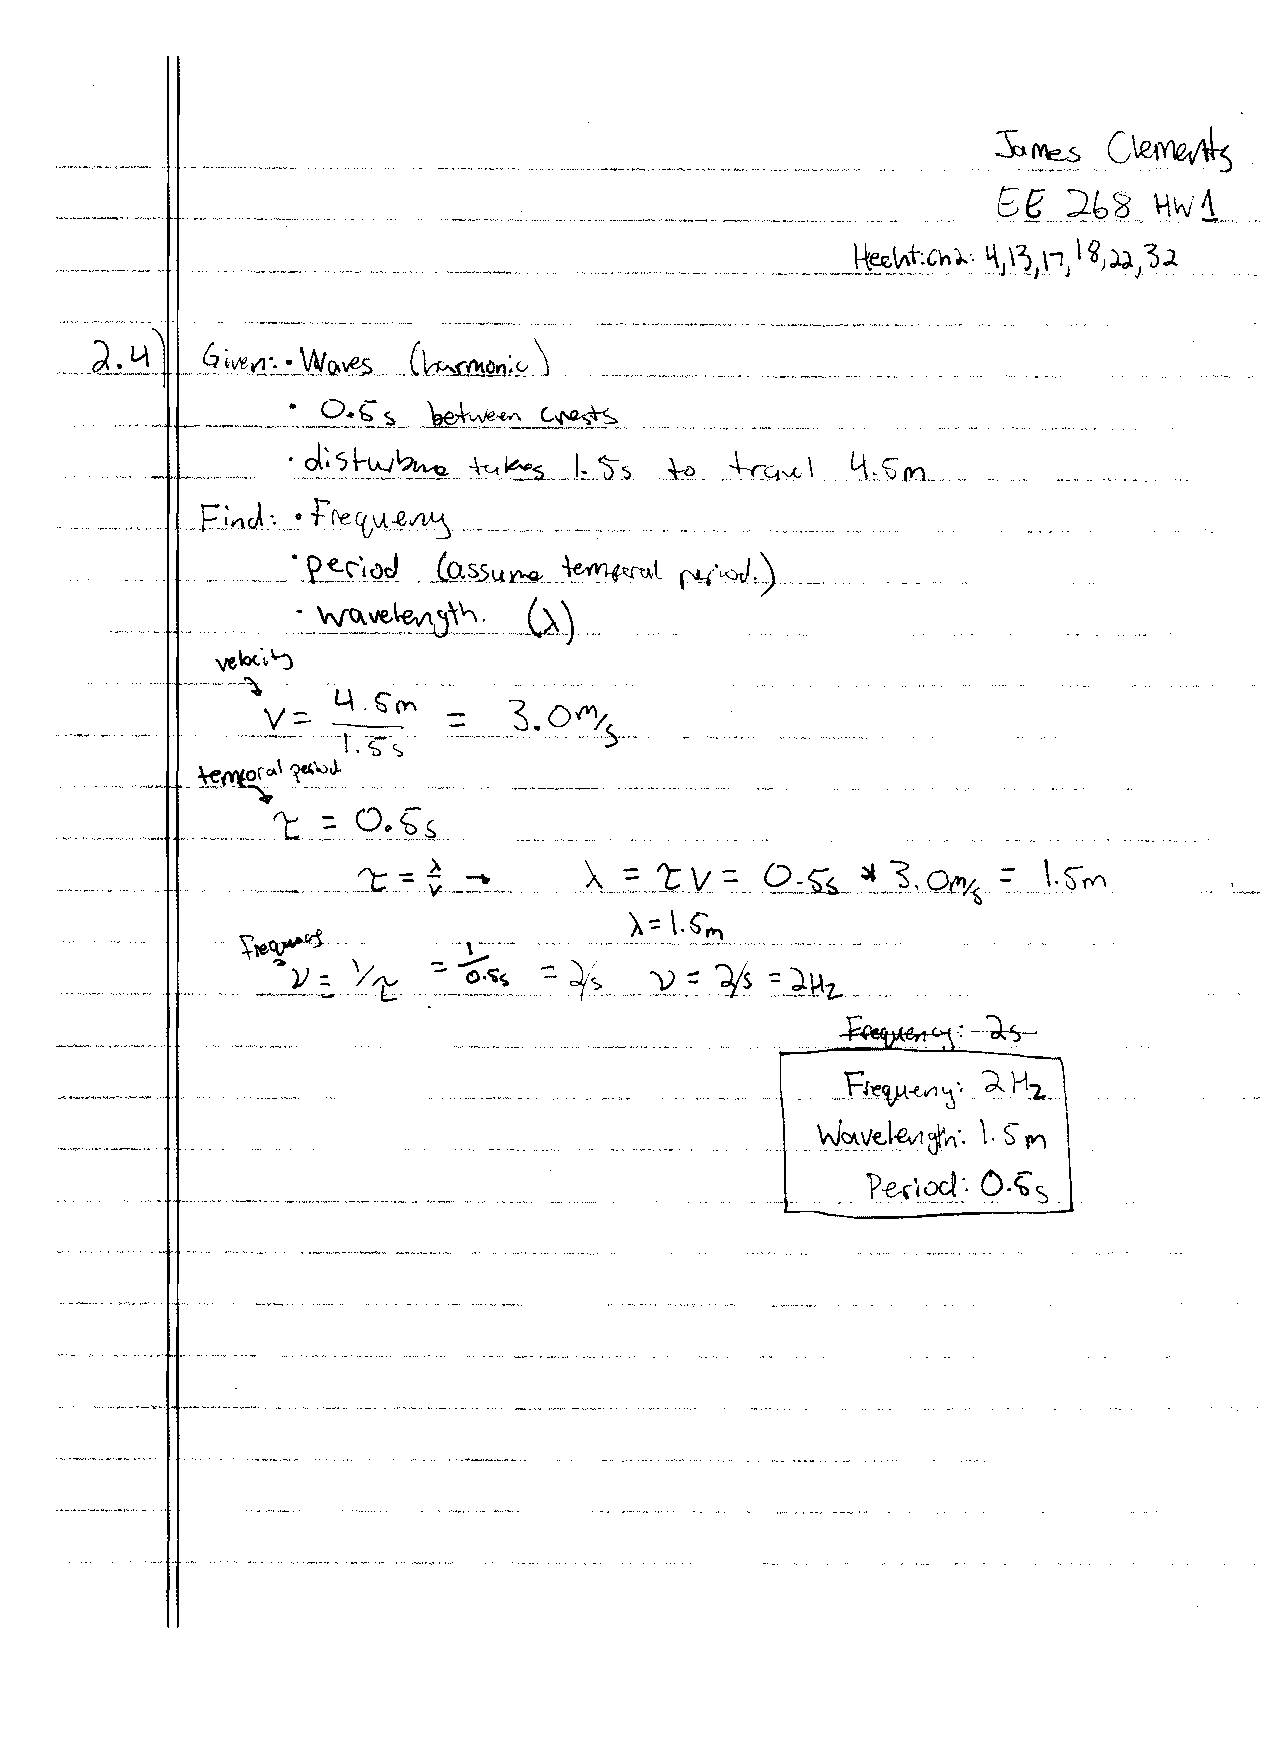
\includepdf[ pages=- ]{EE268HW1}


\chapter{Superposition of Waves}
For certain types of waves, specifically small-amplitude linear systems, the Principle of Superposition is able to be used as a convenient method for determining how multiple waves will interact in a system. The  principle of superpositions suggests that the resultant disturbance at any point in a medium is the algebraic sum of the separate constituent waves. 

\section{Addition of Waves of the Same Frequency}

\subsection{The Algebraic Method}

Take two harmonic electromagnetic waves, $E_1$ and $E_2$, of the form \[E(x,t) = E_0 \sin [ \omega t + \alpha(x,\epsilon)]\]  (where $\alpha(x,\epsilon) = -(kx+\epsilon)$ is used to separate the spatial terms from the temporal terms) are occupying the same place in space such that they interact with one another. By grouping terms the equations can be written out as: 
\[E_1 = E_{01} \sin (\omega t + \alpha_1 )\] \[E_2 = E_{02} \sin (\omega t + \alpha_2 )\]

The resulting disturbance, $E = E_1+E_2$ can be written as:
\begin{equation}
E = E_0 \sin (\omega t + \alpha)
\end{equation}
where
\begin{equation}
E_0 ^2 = E_{01} ^2 + E_{02} ^2 + 2E_{01}E_{02} \cos (\alpha_2 - \alpha_1)
\end{equation}
\begin{equation}
\tan \alpha = \frac{E_{01} \sin \alpha_1 + E_{02} \sin \alpha_2}{E_{01} \cos \alpha_1 + E_{02} \cos \alpha_2}
\end{equation}

The term: $2E_{01}E_{02} \cos (\alpha_2 - \alpha_1)$ is the interference term which contains the crucial phase difference term: \[\delta \equiv (\alpha_2-\alpha_1)\] which can arise from a difference in path length as well as a difference in initial phase angle such that:
\[\delta = (kx_1+\epsilon_1) - (kx_2+\epsilon_2)\]
\[\delta = \frac{2\pi}{\lambda}(x_1-x_2)+(\epsilon_1-\epsilon_2)\]
where $x_1$ and $x_2$ are distances from the sources of the two waves to the point of observation. If the waves are initially in-phase at their sources, then $\epsilon_1 = \epsilon_2$.

When two disturbances from the same source travel different routes before arriving at the point of observation, \[\delta = \frac{2\pi}{\lambda_0}n(x_1-x_2)\] where $n$ is the index of refraction of the medium. $n(x_1-x_2)$ is known as the optical path difference (OPD or $\Lambda$).

Also, when $\epsilon_1-\epsilon_2$ is a constant value, the waves are said to be coherent. For multiple in-phase, coherent sources: \[E_0 ^2 = \left( \displaystyle\sum\limits_{i=1}^N E_{0i} \right)^2 \] which simplifies to the following when all the amplitudes are the same value of $E_{01}$:
\[E_0 ^2 = N^2 E_{01}^2\] whereas for incoherent light: \[E_0 ^2 = N E_{01}^2\]

\subsection{Standing Waves}

A standing wave consists of 2 harmonic waves (possibly a reflection of a wave from the same source) which have the same frequency and period, but travel in opposite directions. A standing wave, or stationary wave, has a profile that does not move through space. Considering a case with two waves, the incident wave: $E_I$, and the reflected wave: $E_R$:
\[E_I = E_{0I} \sin (kx+\omega t+\epsilon_I)\]
\[E_R = E_{0R} \sin (kx+\omega t+\epsilon_R)\]
The boundary condition of the standing wave requires that $\epsilon_1 = \epsilon_2$. Assuming that the amplitudes are the same (that is, $E_{0I} = E_{0R}$) the following equation will represent the resultant wave:
\begin{equation}
E(x,t) = 2E_{0I} \sin kx \cos \omega t
\end{equation}
The point of lowest intensity on a standing wave is called a node, and the point of highest amplitude is an amplitude. These are significant concepts in electromagnetic theory. 

\section{Addition of Waves of Different frequency}
\subsection{Beats}

Beats contain 2 waves at different frequencies traveling in the same direction. They have the same initial phase angles (can assume this to be zero): 
\[E_1 = E_{01} \cos (k_1x - \omega _1 t)\]
\[E_2 = E_{02} \cos (k_2x - \omega _2 t)\]
It can be shown that the total disturbance will take the form if the waves have equal amplitudes and zero initial phase angles:
\begin{equation}
E = 2E_{01} \cos (k_mx-\omega_m t) \cos (\bar{k}x-\bar{\omega}t)
\end{equation}
where
\[\bar{\omega} \equiv \frac{1}{2}(\omega_1+\omega_2)\]
\[\omega_m \equiv \frac{1}{2}(\omega_1-\omega_2)\]
\[\bar{k} \equiv \frac{1}{2}(k_1+k_2)\]
\[k_m \equiv \frac{1}{2}(k_1-k_2)\]
The difference terms are dominated by the low frequency component, whereas the average terms of \textomega {}  and k are dominated by the high frequency component. The low frequency wave profile essentially encompasses the high frequency wave. The low frequency wave moves at the group velocity, $v_g = \frac{\omega_m}{k_1} = \left( \frac{\partial \omega }{\partial k} \right)_{\bar{\omega}}$ whereas the high frequency carrier wave travels at a phase velocity $v_c = \frac{\bar{\omega}}{\bar{k}}$. $\omega(k)$ is the dispertion relation which is a property of the medium. 

\section{Anharmonic Periodic Waves}
Some waves are not harmonic. These are hard to analyzed, so they are instead represented as superpositioning harmonic waves so that they're continuous and differentiable. The Fourier series is commonly used for this. A periodic function $f(x)$ can be represented by the following series:
\begin{equation}
f(x) = \frac{A_0}{2}+ \displaystyle\sum\limits_{m=1}^\infty A_m \cos mkx + \displaystyle\sum\limits_{m=1}^\infty B_m \sin mkx
\end{equation}
where
\begin{equation}
A_0 = \frac{2}{\lambda} \int_0^\lambda f(x)dx
\end{equation}
\begin{equation}
A_m = \frac{2}{\lambda}\int_0^\lambda f(x) \cos mkx dx
\end{equation}
\begin{equation}
B_m = \frac{2}{\lambda}\int_0^\lambda f(x) \sin mkx dx
\end{equation}

This Fourier Series Analysis business can be extrapolated into two dimensions for the discrete Fourier transform which is commonly used in image processing. 
\section{Nonperiodic Waves}
Nonperiodic waves do not repeat continuously. This makes Fourier series somewhat of an awkward tool to use for analysis. The Fourier integral was designed to handle such signals which are often caused by pulses and wave packets. The governing equations of the Fourier integral are as follows:
\begin{equation}
f(x) = \frac{1}{\pi} \left[ \int _0^\infty A(k) \cos kx dk + \int_0^\infty B(k) \sin kxdk \right]
\end{equation}
where:
\begin{equation}
A(k) = \int_{-\infty}^\infty f(x) \cos kxdx
\end{equation}
\begin{equation}
B(k) = \int_{-\infty}^\infty f(x) \sin kxdx
\end{equation}

\section{Glossary}
\begin{description}
\item[Absorption band:] The wavelength band within which materials absorb electromagnetic energy.
\item[Anomalous dispersion:] When the group velocity is greater than the carrier velocity in a system of waves with multiple frequencies. 
\item[Coherence length:] The spatial length in which a wave remains within its frequency bandwidth. 
\item[Coherence time:] The time in which a wave remains in its allocated frequency bandwidth. 
\item[Coherent:] Waves are coherent when their initial phase difference $\varepsilon_1-\varepsilon_2 = a$ where $a$ is a constant.
\item[Constructive interference:] Occurs when interference among waves causes an overall increase in the intensity of the disturbance. 
\item[Destructive interference:] When the interference between waves causes an overall decrease in intensity of the distrubance. 
\item[Dispersive medium:] A medium in which the phase velocity of a wave or group of waves depends on its frequency. 
\item[Group velocity:] The velocity of some shape or leading edge of a pulse, it is taken as the rate at which a feature moves to be the velocity of the group of waves as a whole. 
\item[Normal dispersion:] When group velocity is less than the carrier velocity of waves with multiple frequencies. 
\item[Optical path difference (OPD):] The difference in two optical paths, $n(x_1-x_2)$
\item[Power spectrum:]  A measure of the distribution of energy, or power, at each and every component frequency that has been analyzed using a discrete Fourier transform.
\item[Standing or Stationary wave:] A wave whose profile does not move through space.
\item[Wave packet:] A small part of a wavetrain. One pulse of a wavetrain specifically that assemble together as a continuous range of spatial frequencies. 
\end{description}

\section{Useful Equations}
Sum of 2 waves: 
\begin{equation}
E = E_0 \sin (\omega t + \alpha)
\end{equation}
\begin{equation}
E_0 ^2 = E_{01} ^2 + E_{02} ^2 + 2E_{01}E_{02} \cos (\alpha_2 - \alpha_1)
\end{equation}
\begin{equation}
\tan \alpha = \frac{E_{01} \sin \alpha_1 + E_{02} \sin \alpha_2}{E_{01} \cos \alpha_1 + E_{02} \cos \alpha_2}
\end{equation}

Fourier Series:
\begin{equation}
f(x) = \frac{1}{\pi} \left[ \int _0^\infty A(k) \cos kx dk + \int_0^\infty B(k) \sin kxdk \right]
\end{equation}
where:
\begin{equation}
A(k) = \int_{-\infty}^\infty f(x) \cos kxdx
\end{equation}
\begin{equation}
B(k) = \int_{-\infty}^\infty f(x) \sin kxdx
\end{equation}

\chapter{Electromagnetic Theory, Photons, and Light}
\section{Basic Laws of Electromagnetic Theory}
This is pretty much review from electricity and magnetism from undergrad physics. Specifically, Faraday's Induction Law (changing magnetic field generates current), Gauss's Laws (electric and magnetic flux), and Ampere's Circuital law (time varying current creates magnetic field). 

Maxwells equations sum up the results of Faraday, Gauss, and Ampere. In derivative form, they are as follows: 

\begin{equation}
\begin{array}{c}
\displaystyle \frac{\partial\vec{E}_z}{\partial y} - \frac{\partial\vec{E}_y}{\partial z} = \frac{\partial\vec{B}_x}{\partial t} \\
\displaystyle\frac{\partial\vec{E}_x}{\partial z} - \frac{\partial\vec{E}_z}{\partial x} = \frac{\partial\vec{B}_y}{\partial t} \\
\displaystyle\frac{\partial\vec{E}_y}{\partial x} - \frac{\partial\vec{E}_x}{\partial y} = \frac{\partial\vec{B}_z}{\partial t}
\end{array}
\end{equation}
\begin{equation}
\begin{array}{c}
\displaystyle\frac{\partial\vec{B}_z}{\partial y} - \frac{\partial\vec{E}_y}{\partial z} = \mu_0\epsilon_0 \frac{\partial\vec{E}_x}{\partial t} \\
\displaystyle\frac{\partial\vec{B}_x}{\partial z} - \frac{\partial\vec{E}_z}{\partial x} = \mu_0\epsilon_0 \frac{\partial\vec{E}_y}{\partial t} \\
\displaystyle\frac{\partial\vec{B}_y}{\partial x} - \frac{\partial\vec{E}_x}{\partial y} = \mu_0\epsilon_0 \frac{\partial\vec{E}_z}{\partial t}
\end{array}
\end{equation}

\begin{equation}
\frac{\partial\vec{B}_x}{\partial x}+\frac{\partial\vec{B}_y}{\partial y}+\frac{\partial\vec{B}_z}{\partial z} = 0
\end{equation}

\begin{equation}
\frac{\partial\vec{E}_x}{\partial x}+\frac{\partial\vec{E}_y}{\partial y}+\frac{\partial\vec{E}_z}{\partial z} = 0
\end{equation}

\section{Electromagnetic Waves}
As their name implies, electromagnetic waves are combinations of both electric fields propagating with a magnetic field. Visible light is a small part of the spectrum of electromagnetic waves. The magnetic disturbance and the electric disturbance always travel perpendicular to one another.  

\section{Energy and Momentum}
Electromagnetic waves are capable of altering energy of all types (including kinetic) of materials they come across. The pointing vector is used to descrive the propagation of a wave and the power per unit area crossing a surface for a wave. 
\begin{equation}
\vec{S} = c^2\epsilon_0 \vec{E}\times\vec{B}
\end{equation}
Where $\vec{S}$ is the Poynting vector, c is the speed at which a wave propagates, $\epsilon_0$ is the permativity of free space, and E and B describe the electric and magnetic fields respectively. 

The time-averaged value of the magnitude of this poynting vector ($\langle S \rangle_T$ is a measure of the irradiance, $I$.
\begin{equation}
I \equiv \langle S \rangle _T = \frac{c\epsilon_0}{2}E_0^2 = \frac{c}{\mu_0} \langle B^2 \rangle_T = \epsilon_0 c \langle E^2 \rangle_T
\end{equation}

Photons carry electromagnetic energy. It is often useful to think of the flow (or flux) of many photons instead of just 1. The mean photon flux is :
\[\Phi = AI/h\nu_0 = P/h\nu_0\]

The energy in a flow of photons is capable of exerting minimal amounts of pressure on objects in a direction that is normal to the propagation vector of the wave. This is the instantaneous pressure that would be exerted on a perfectly absorbing surface by a normally incident beam. The average radiation pressure is expressed as:
\begin{equation}
\langle \mathcal{P}(t) \rangle_T = \frac{\langle S(t) \rangle_t}{c} = \frac{I}{c}
\end{equation}
This same pressure is exerted on a source that is radiating energy 

\section{Radiation}
There are a lot of really cool things that can be done with radiation (such as optical cooling). In general, the rule when dealing with radiation is that Energy is most strongly radiated perpendicular to the acceleration causing it. 

\section{Light in Bulk Matter}
The phase speed in a medium is:
\[v = 1/\sqrt{\epsilon\mu}\]
The ratio of the speed of an electromagnetic wave in vacuum to that in matter is the absolute index of refraction, $n$:
\begin{equation}
n \equiv \frac{c}{v} = \sqrt{\frac{\epsilon \mu}{\epsilon_0 \mu_0}}
\end{equation}

\section{The Electromagnetic-Photon Spectrum}
This is section review from most early science courses. The common forms of electromagnetic energy from low energy to high energy waves are: radio waves, microwaves, ifrared, light, ultraviolet, x-rays, and gamma rays.

\section{Glossary}
\begin{description}
\item[Dielectric constant: ] Symbolically $K_E = \epsilon/\epsilon_0$. Also known as the relative permittivity of a material. 
\item[Electric permittivity: ] The electrical behavior of a medium. The degree to which the material is permeated by the electric field in which it is immersed. 
\item[Energy density: ] The radiant energy per unit volume of some region of space. ($u$)
\item[Exitance: ]
\item[Index of refraction: ] The ratio of the speed of an electromagnetic wave in vacuum to that in matter. 
\item[Irradiance: ] The average energy per unit area per unit time from a light source on a surface. 
\item[Maxwell's equations: ] Equations that describe the interactions between electricity and magnetism. 
\item[Photon flux: ] The number of photons passing through a unit area. 
\item[Optical power: ] The time rate of flow of radiant energy ($P$)
\item[Orientational polarization: ]
\item[Permeability: ] The ease at which mass moves through a medium. 
\item[Photon: ] Stable, chargeless, massless elementary particles that exist only at the speed $c$. 
\item[Polarization: ] The moment-by-moment direction of an electric field carried by an electromagnetic wave. 
\item[Poynting vector: ] A vector that describes the power per unit area of a wave crossing a surface 
\item[Radiation pressure: ] The pressure exerted on a surface normal to the propagation of an electromagnetic wave.
\item[Relative permeability: ] The amount compared to the permeability of free space that a medium is permeable. 
\item[Resonance frequency: ] The frequency at which the energy of the photon exactly matches the quantized energy decrease of the atom at $\mathcal{E} = h\nu$. Atoms very efficiently absorb and emit energy by shifting electrons at their resonant frequency. 

\end{description}
\section{Useful Equations}
\[\begin{array}{c}
\displaystyle \frac{\partial\vec{E}_z}{\partial y} - \frac{\partial\vec{E}_y}{\partial z} = \frac{\partial\vec{B}_x}{\partial t} \\
\displaystyle\frac{\partial\vec{E}_x}{\partial z} - \frac{\partial\vec{E}_z}{\partial x} = \frac{\partial\vec{B}_y}{\partial t} \\
\displaystyle\frac{\partial\vec{E}_y}{\partial x} - \frac{\partial\vec{E}_x}{\partial y} = \frac{\partial\vec{B}_z}{\partial t}
\end{array}\]
\[\begin{array}{c}
\displaystyle\frac{\partial\vec{B}_z}{\partial y} - \frac{\partial\vec{E}_y}{\partial z} = \mu_0\epsilon_0 \frac{\partial\vec{E}_x}{\partial t} \\
\displaystyle\frac{\partial\vec{B}_x}{\partial z} - \frac{\partial\vec{E}_z}{\partial x} = \mu_0\epsilon_0 \frac{\partial\vec{E}_y}{\partial t} \\
\displaystyle\frac{\partial\vec{B}_y}{\partial x} - \frac{\partial\vec{E}_x}{\partial y} = \mu_0\epsilon_0 \frac{\partial\vec{E}_z}{\partial t}
\end{array}\]
\[\frac{\partial\vec{B}_x}{\partial x}+\frac{\partial\vec{B}_y}{\partial y}+\frac{\partial\vec{B}_z}{\partial z} = 0\]
\[\frac{\partial\vec{E}_x}{\partial x}+\frac{\partial\vec{E}_y}{\partial y}+\frac{\partial\vec{E}_z}{\partial z} = 0\]
\[\vec{S} = c^2\epsilon_0 \vec{E}\times\vec{B}\]
\[I \equiv \langle S \rangle _T = \frac{c\epsilon_0}{2}E_0^2 = \frac{c}{\mu_0} \langle B^2 \rangle_T = \epsilon_0 c \langle E^2 \rangle_T\]
\[\langle \mathcal{P}(t) \rangle_T = \frac{\langle S(t) \rangle_t}{c} = \frac{I}{c}\]
\[v = 1/\sqrt{\epsilon\mu}\]
\[n \equiv \frac{c}{v} = \sqrt{\frac{\epsilon \mu}{\epsilon_0 \mu_0}}\]


\chapter{Polarization}
\section{The nature of polarized light}
Light in this text has previously been considered to be linearly polarized or plane-polarized. In this case, the orientation of the electrical field is constant, but it's magnitude as sign can vary in time. This disturbance occurs in a plane called a plane of vibration which is a fixed plane containing the electric field and propagation vectors. 

Light waves can also act in such a way that their electric field orientations are mutually perpendicular. The superposition of these waves may not be linearly polarized as they are when 2 linearly polarized waves interact. 

\subsection{Linear Polarization}
Two orthogonal optical waves can be represented as:
\[\vec{E}_x(z,t)=\hat{i}E_{0x} \cos (kz-\omega t)\]
\[\vec{E}_y(z,t)=\hat{j}E_{0y} \cos (kz-\omega t+\varepsilon)\]
where $\varepsilon$ is the relative phase difference between the waves which are both traveling in the z-direction. The resultant wave when the two are in phase is:
\[\vec{E}=(\hat{i}E_{0x}+\hat{j}E_{0y}) \cos (kz-\omega t)\]
This wave is linearly polarized on a plane that is some angle between the x-z and y-z planes. 

If $\varepsilon$ is an odd integer multiple of $\pi$ such that the waves are 180 degrees out of phase then the resulting equation becomes:
\[\vec{E}=(\hat{i}E_{0x}-\hat{j}E_{0y}) \cos (kz-\omega t)\] which is a rotated version of the previous equation. 

\subsection{Circular Polarization}
When both waves have the same amplitude, yet vary in phase by some form of $\pm \frac{\pi}{2}$, they are said to be circularly polarized. The two waves resemble:
\[\vec{E}_x(z,t)=\hat{i}E_{0x} \cos (kz-\omega t)\]
\[\vec{E}_x(z,t)=\hat{i}E_{0x} \sin (kz-\omega t)\]
and form a consequent waves:
\[\vec{E} = E_0 \left[\hat{i} \cos (kz-\omega t) +\hat{j}\sin (kz-\omega t) \right]\]
When light moving toward an observer is rotating clockwise, the wave is called right-circularly clockwise. Similarly, a wave rotating counter clockwise as it travels toward an observer is left-circularly polarized. In circularly polarized light, the endpoint travels in a circle around the axis that the wave is traveling at a rate of 1 rotation per wavelength. 
\subsection{Elliptical Polarization}
Both linear and circular polarized light are types of elliptical polarization (they're at the extremes of the light). This type of polarization is when the end location of light travels in an ellipse on a plane perpendicular to the propagation vector. This is the case when the equation describing the two waves are independent in of space or time (the kz - \textomega t is gone). The equations mentioned so far in this chapter can be altered to the form:
\begin{equation}
\left( \frac{E_y}{E_{0y}} \right) ^2 + \left( \frac{E_x}{E_{0x}} \right) ^2 -2 \left( \frac{E_x}{E_{0x}} \right) \left( \frac{E_y}{E_{0y}} \right) \cos \varepsilon = \sin ^2 \varepsilon
\end{equation}

Which is a plane making angle \textalpha with the $(E_x,E_y)$-coordinate system such that:
\begin{equation}
\tan 2\alpha = \frac{2E_{0x}E_{0y}\cos \varepsilon}{E_{0x}^2 - E_{0y}^2}
\end{equation}

The state of polarization can be linearly/planarly plarized in a $\mathcal{P}$-state, it can be right or left circularly polarized in an $\mathcal{R}$ or $\mathcal{L}$ state, and finally is can be in a state of elliptical polarization which is designated as an $\mathcal{E}$ state. 

\subsection{Natural light}
Light sources which emit random rapidly varying successions of different polarization states are referred to as natural light (also as unpolarized light). Light found in nature and man-made light are neither made completely of polarized or completely unpolarized lights. The electric field vector usually varies in what is known as being partially polarized. Do note that the infinite nature of monochromatic light causes it to be perfectly polarized.

\subsection{Angular Momentum and Photon Picture} 
Electromagnetic waves apply energy and linear momentum to bodies they encounter. Power delivered to system by an electromagnetic wave is measured in energy transferred per unit time, $d\mathcal{E}/dt$. The power generated by a torgue, \textGamma, acting on a rotating body is $\omega\Gamma$ (or $vF$ for linear motion), such that:
\[\frac{d\mathcal{E}}{dt}=\omega\Gamma\]
Torque is equal to the time rate-of change of angular momentum, L, so that on average:
\[\frac{d\mathcal{E}}{dt}=\omega\frac{dL}{dt}\]
A charge that absorbs a quantity of energy from the incident circular wave simultaneously absorbs angular momentum L so:
\[L=\frac{\mathcal{E}}{\omega}\]


\section{Polarizers}
Any device that takes an input of unpolarized light and outputs a form of polarized light is called a polarizer. Polarizers use one of the following physical mechanisms: dichroism (selective absorption), reflection, scattering, and birefrengence (double refraction). There is asymmetry involved with all of these processes. 
\subsection{Malus's Law}
This is involved in experimentally determining if a device is a (linear) polarizer. 

The $\mathcal{P}$-state of a wave emerging from a linear polarizer will have an orientation parallel to what is defined as the transmission axis of a polarizer. Only the component of the optical field parallel to the transmission axis will pass through the device unaffected. An analyzer is a second polarizer that is put into an optical train to test the polarization of the other polarizing device. The irradiance reaching a detector behind both devices is given by:
\[I(\theta) = \frac{c\epsilon_0}{2}E_{01}^2\cos ^2 \theta\] 
Maximum irradiance occurs when the angle between the transmission axes of the analyzer and polarizer is zero, I(0). This leads to Malus's Law which is:
\begin{equation}
I(\theta)=I(0)\cos^2\theta
\end{equation}
where I(0) is the irradiance arriving at the analyzer:
\begin{equation}
I(0) = c\epsilon_0E_{01}^2/2
\end{equation}
Be aware that nonideal polarizers only work within a certain range of wavelengths. 
\subsection{Dichroism}
Dichroism is the selective absorption of one of the two orthogonal $\mathcal{P}$-state components of an incident beam. Dichroic polarizers are physicially anisotropic producing an asymmetric absorption of one field component and remaining transparent to the other. 
\subsection{Birefringence}
An anisotropy in the binding force between atoms in a crystal lattice will be manifest in an anisotropy in the refractive index. This is because the speed of the wave (which is related to index of refraction) is the difference between the frequency of the $\vec{E}$-field and the natural frequency of the atoms. A material that displays two different indices of refraction is defined to be birefringent. 

The optic axis is a direction through which a material has one index of refraction and is perpendicular to 2 other directions of another index of refraction. The direction of the optic axis corresponds to a special crystallographic orientation which is an axis of 3-fold symmetry. 

In a birefrengent crystal such as calcite. Rays  traveling through it as if they had passed through a plate of glass are known as ordinary rays (o-rays). Ordinary rays will not rotate along with a crystal. Rays that are affected by rotation of a crystal are extraordinary rays. Ordinary and extraordinary waves are both polarized and are perpendicular to one another. 

\subsection{Scattering and polarization}
Particles around the same size as light scatter it in many different directions. Unpolarized light entering a medium with scattering particles can be scattered at angles normal to the incident light's propagation vector. The scattered light in the forward direction is completely unpolarized.  

\subsection{Polarization by reflection}
Reflecting from dielectric (insulating) media is a common source of polarized light. Forms of glare from windows, paper, and other insulating types of material are partially polarized. For an electron-oscillator: the incoming polarized wave made up of 2 incoherent orthogonal $\mathcal{P}$-states, only the component polarized normal to the incident plane and therefore parallel to the surface will be reflected. The angle of incidence for which this occurs is $\theta_p$ which is the polarization angle or Brewster's angle where $\theta_p+\theta_t=90^\circ$. From Snell's Law:
\begin{equation}
n_i \sin \theta_p = n_t \sin \theta_t
\end{equation}
The fact that $\theta_t = 90^\circ - \theta_p$ leads to Brwster's Law:
\begin{equation}
\tan \theta_p = n_t/n_i
\end{equation}
where the subscript "i" refers to the incident beam and the properties of its medium, the subscript "t" refers to the same for the transmitted beam, and the subscript "p" refers to polarization. 

The Fresnel equations lead to a desirable concept of the degree of polarization V, defined as:
\begin{equation}
V = \frac{I_p}{I_p+I_n}
\end{equation}
where $I_p$ and $I_n$ are the constituent flux densities of the polarized and "unpolarized" natural light. This gives a quantitative way to described how polarized light is. 

\section{Retarders}
A retarder is an optical element which serves to change the polarization of an incident wave. A wave of a certain polarization goes in and a wave with a different type of polarization goes out. This is accomplished by changing the relative phase of the incident beam. 

If an optic axis of a uniaxial crystal (ie calcite) is arranged to be parallel to the front and back surfaces and the incident monochromatic plane wave's $\vec{E}$-field has components parallel and perpendicular to the optic axis, then two separate plane waves will propagate through the crystal. Since $v_\parallel>v_\perp$ and $n_o>n_e$: the e-wace will move across the specimen faster than the o-wave. After traveling a plate of thickness, $d$, the resultant wave has a relative phase difference of $\Delta\varphi$ (these are harmonic waves of the same frequency with orthogonal electric fields. 

The relative optical path length difference is:
\[\Lambda = d(|n_o-n_e|)\]
since $\Delta\varphi = k_0\Lambda$, the phase difference (measured in radians) is:
\begin{equation}
\Delta\varphi=\frac{2\pi}{\lambda_0}d(|n_o-n_e|)
\end{equation}
where $\lambda_0$ is the wavelength in vacuum. 

Some types of retarders: zero order retarder has the minimum thickness necessary to produce a phase difference. Multiple order retarder has a thickness corresponding to a whole number of $2\pi$ shifts plus the phase difference. Compound zero-order wave plates combine the fast axis of one retarder with the slow axis of another to compensate for temperature variations. 

\subsection{The Full-Wave Plate}
When the relative retardation or retardance, $\Delta\varphi = 2\pi$, the optical component is called a full-wave plate or full-wave retarder. Retarders of this sort only work for a narrow range of wavelengths. When the velocity of light parallel to the optic axis is faster than in the perpendicular direction, the optic axis is then referred to as the fast axis. The slow axis is then the perpendicular direction to the optic direction. For materials in which $v_\perp > v_\parallel$, the names are switched (since the perpendicular direction is now faster). 

These are used to eliminate inadvertent changes in polarization state of light passing through an optical system.

\subsection{The Half-Wave Plate}
A retardation plate with retardance of $\pi$ radians between the o-waves and e-waves. These are often made of polyvinyl alcohol sheets or cellophane tape on a microscope slide. For this case, the thickness of the material satisfies:
\[ d(| n_o - n_e |) = (2m+1)\lambda_0 /2\]
where $m$ is an integer. 

\subsection{The Quarter-Wave Plate}
A retarder with retardance, $\Delta\varphi = \pi/2$. Crude quarter wave plates can be made from plastic food wrap. Commercial quarter-wave plates are used for their linear retardation. For this case, the thickness of the material must satisfy: 
\[ d(| n_o - n_e |) = (4m+1)\lambda_0 /4\]
\subsection{Fresnel Rhomb}
The Fresnel rhomb causes a beam to be internally reflected twice, thus imparting a $90^\circ$ relative phase shift. These are almost achromatic 90 degree retarders. 

\subsection{Compensators and Variable Retarders}
A compensator is an optical device that is capable of impressing a controllable retardance on a wave. A common type of compensator, the Babinet compensator uses two triangular wedges to vary the thickness of calcite that a wave will travel through. The total phase difference (retardance) of these devices is:
\[\Delta\varphi=\frac{2\pi}{\lambda_0}(d_1-d_2)(|n_o-n_e|)\]
\section{Circular polarizers}
A series combination of an appropriately oriented linear polarizer and a 90 degree retarder will perform as a circular polarizer. both $\mathcal{L}$ and $\mathcal{R}$ states can be achieved by varying the transmission axis of the linear polarizer at positive 45 degrees or negative 45 degrees measured to the fast axis of the retarder. 
\section{Optical Activity}
Any material that causes an $\vec{E}$-field of an incident linear plane wave to appear to rotate is deemed optically active. There are different types of optical activity in materials. Dextrorotary (d-rotary) and levorotary (l-rotary) and circularly birefringent are common types of optical activity in materials. The rotary power is the degree at which materials are optically active. The phenomenon has to do with the chirality of a crystal structure and is fairly complicated. 

\section{Induced Optical Effects - Optical Modulators}
Interaction with optical mediums often change their properties. 
\subsection{Photoelasticity (stress birefringence)}
Stress birefringence is the phenomenon exhibited when a normally transparent isotropic substance is made anisotropic by the application of mechanical stress. Cartilage for example exhibits stress birefringence. This property is often used as a tool to measure stress within a material. 

\subsection{The Faraday Effect}
The Farady Effect explains the influence of a magnetic field on light. The angle of rotation thorugh which the plane of vibration rotates when it encounters a magnetic field, $\beta$, is expressed empirically as:
\begin{equation}
\beta = \mathcal{V}Bd
\end{equation}
where B is the static magnetic flux density, d is the length of the medium traversed, and $\mathcal{V}$ is the Verdet constant which is particular to a medium and varies with frequency and temperature. 
\subsection{The Kerr and Pockels Effects}
The Kerr effect explains how an electric field can make a normally isotropic transparent material birefringent like a uniaxial crystal with an optic axis that corresponds to the direction of the applied field. The difference in indeces of refraction is known to be:
\[\Delta n = n_e-n_o = \lambda_0KE^2\] where K is the Kerr constant, E is the magnitude of the electric field,  $\lambda_0$ is the wavelength in vacuum. Digital shutters for cameras often make use of the Kerr effect. 

The Pockels Effect is similar to the Kerr effect in which crystals that lack a center of symmetry can have their optics modified. It is more sensitive than the Kerr effect and the cells are easier to manage. 

\section{Liquid Crystals}
 Liquid crystals are a phase of matter that interact with light in a away that is hybrid between liquids and solids. There are three types of crystals that are differentiated by molecular alignment. Nemetic liquid crystals contain molecules that are randomly positioned, yet mostly parallel. These can be manipulated for many purposes including inducing controllable birefringence and the making of displays on screens. 
\section{A Mathematical Description of Polarization}
 \subsection{The Stokes Parameters}
 The Stokes parameters are four quantities that are functions only of observables of the electromagnetic wave. The polarization state of light can be described in terms of these quantities. In an experimental setup, suppose that the first filter is isotropic, the scond and thierd are linear polarizers with transmission axes orizontal and at +45 degrees, the last filter is a circular polarizer. The transmitted irradiances, $I_0, I_1, I_2, I_3$ (in order of the polarizers on the optical train) are used to define the Stokes parameters. 
 
\[\mathcal{S}_0 = 2I_0\]
\[\mathcal{S}_1 = 2I_1-2I_0\]
\[\mathcal{S}_2 = 2I_2-2I_0\]
\[\mathcal{S}_3 = 2I_3-2I_0\]

$\mathcal{S}_0$ is the incident irradiance, and the other parameters specify the state of polarization. The stokes parameters are often grouped as a column vector, $\vec{\mathcal{S}}$.
\subsection{The Jones Vectors}
The Jones Vectors are another representation of polarized light that are only applicable to polarized waves. The Jones vector in column form is comprised of the instantaneous scalar components (x and y) of the electric field. The Jones vector is defined as:

\[\vec{E} = \left[\begin{array}{c}
E_x(t) \\
E_y(t) \\

\end{array} \right]\]
\subsection{Jones and Mueller Matrices}
These matrices are used to model the transformation of light as it travels through a polarizing element. The Mueller matrices were devised as a method for dealing with Stokes vectors. The Mueller ma

\section{Glossary}
\begin{description}
\item[Analyzer: ] A second polarizer in an optical train used to test another polarizer. Often a mostly ideal linear polarizer is used for this purpose. 
\item[Birefringence: ] the material property referring the the display of two different indices of refraction. Mathematically defined as $\Delta n = n_e - n_o$ where $n_e$ and $n_o$ are the index of refraction of the extraordinary arrays and the ordinary rays, respectively. 
\item[Brewster's angle: ] The polarization angle $\theta_p$ in which the reflected angle and transmitted angle from an incident beam onto a surface is equal to 90 degrees. 
\item[Circular birefringence: ] a property of materials that posess two indices of refraction. One for $\mathcal{R}$- and one for $\mathcal{L}$-states. Denoted $n_\mathcal{R}$ and $n_\mathcal{L}$
\item[Circularly polarized: ] A result of multiple waves traveling to an observer that appear to rotate circularly on a plane perpendicular to the axis of propagation. 
\item[Cleavage plane: ] Smooths surfaces on which a material can be easily split.
\item[Compensator: ] An optical device that is capable of impressing a controllable retardance on a wave.
\item[Dichroism: ] The selective absorption of one of the two orthogonal $\mathcal{P}$-state components of an incident beam.
\item[Extraordinary ray: ] A ray that rotates with a birefringent crystal. 
\item[Faraday effect: ]The manner in which light propageted through a material medium could be influenced by the application of an external magnetic field. 
\item[Fast axis: ] The axis in a wave plate in which waves travel fastest. 
\item[Half-wave plate: ] A wave plate with retardance of $\pi$ radians.
\item[Jones vector: ] A representation of polarized light that is only applicable to polarized waves. 
\item[Kerr effect: ] The effect in which an electric field $\vec{E}$ causes a material to become birefringent. 
\item[Liquid Crystal: ] A phase of matter that possesses physical properties between those of ordinary liquids and solids. 
\item[Malus's law: ] $I(\theta)=I(0)\cos^2\theta$
\item[Mueller matrix: ] A transformation matrix which handles the Stokes vectors and can thus handle polarized and partially polarized light. These are 4x4 matrices unlike the Jones matrix which is 2x2. 
\item[Optic axis: ] The direction in a birefrengent crystal through which light travels through one index of refraction and has a crystal such that the 2 perpendicular directions to the Optic axis direction are of another index of refraction. 
\item[Optical activity: ] the phenomenon in which a material causes the elctric field of an incident linear plane wave to appear to rotate.
\item[Ordinary ray: ] A ray that is unaffected by the rotation of a birefringent crystal.
\item[Polarization state: ] describes if light is in a: linear or planar $\mathcal{P}$-state; right or left circularly polarized in an $\mathcal{R}$ or $\mathcal{L}$ state; or in a state of elliptical polarization which is designated as an $\mathcal{E}$ state. 
\item[Retarder: ] An optical element that changes the polarization of an incident wave.
\item[Stress birefringence: ] The phenomenon exhibited when a normally transparent isotropic substance is made anisotropic by the application of mechanical stress.
\item[Stokes parameters: ] 4 parameters designated by $\mathcal{S}_{0,1,2,3}$ that describe incident light and it's polarization state. 
\item[Transmission axis: ] The axis to which the light traveling out of a polarizer is parallel. 
\item[Twisted nematic cell: ] A nemetic cell which has molecular layers that spiral about an axis. This is typically done in layers. 
\item[Uniaxial crystal: ] A crystal in which there is only one direction about which atoms are arranged symmetrically. 
\item[Unpolarized light: ] Also known as natural light. A disturbance from a source that emits randomly polarized wave packets. 

\end{description}

\section{Useful Equations}
\[\left( \frac{E_y}{E_{0y}} \right) ^2 + \left( \frac{E_x}{E_{0x}} \right) ^2 -2 \left( \frac{E_x}{E_{0x}} \right) \left( \frac{E_y}{E_{0y}} \right) \cos \varepsilon = \sin ^2 \varepsilon\]
\[\tan 2\alpha = \frac{2E_{0x}E_{0y}\cos \varepsilon}{E_{0x}^2 - E_{0y}^2}\]
\[I(\theta)=I(0)\cos^2\theta\]
\[I(0) = c\epsilon_0E_{01}^2/2\]
\[n_i \sin \theta_p = n_t \sin \theta_t\]
\[\tan \theta_p = n_t/n_i\]
\[V = \frac{I_p}{I_p+I_n}\]
\[\Delta\varphi=\frac{2\pi}{\lambda_0}d(|n_o-n_e|\]
\[\beta = \mathcal{V}Bd\]

\chapter{Interference}
\chapter{Modern Optics - Lasers and Such}



\part{Light and Matter}

\chapter{The Propagation of light}
The processes of transmission, reflection, and refraction are macroscopic manifestations of scattering occurring on a submicroscopic level. 
\section{Rayleigh Scattering}
Rayleigh scattering is the process in which particles that are smaller than the wavelength of light, less than approximately $\lambda/15$, are scattered. Light that closer to the resonant frequency of the particles scatters more than light with a distance frequency. This process is behind most blues found in organisms. The sky is blue for similar reasons, but is slightly different as it relies on random density fluctuations in the mid-atmosphere.
\subsection{Scattering and Interference} 
The denser the substance through which light advances, the less the lateral scattering. 

Random, widely spaced scatterers driven by an incident primary wave emit wavelets that are essentially independent of one another in all directions except forward. Laterally scattered light, unimpeded by interference, streams out of the beam. This approximately happens in the upper atmosphere (100 miles above sea level). 
\paragraph{Forward Propagation}
Beams of light are mostly undisturbed in the forward direction because they constructively interfere as they travel in that direction (for the most part). All scattered wavelets add constructively with each other in the forward direction because of the asymmetry introduced by the beam. 
\subsection{The Transmission of Light Through Dense Media}
When light travels through dense media, scattered wavelets still interfere constructively in the forward direction, but now desctructive interference predominates in other directions. Little or no  light ends up scattered laterally or backwards in a dense homogeneous medium. 

Interference produces a redistribution of energy, out of the regions where it is destructive and into regions where it is constructive. 

More order in a substance leads to less scattering. 
\subsection{Transmission and the Index of Refraction}
Even through photons only exist at a speed $c$, light through a medium travels at a different speed. This ratio is the index of refraction ($n = c/v$) where n is the index of refraction, c is the speed of light in vacuum, and v is the velocity of the light in question. This is brought about by the material phase shifting the light as it travels through the medium. Phase shift is essentially related to a shift in phase velocity. 

The index of refraction arises when the absorption and emission process advances or retards the phases of the scattered photons, even as they travel at speed $c$.

Therefore, a light wave propagating through any substantive medium travels at a speed $v \neq c$

\section{Reflection}
Drastic changes in the dielectric constant (or index of refraction) cause much reflection, small changes induce less. Gradual changes cause less changes as well. The characteristic length in question here is wavelength. Changes larger than a wavelength are gradual, less than are sudden. 

The layer of scatters that primarily cause reflection are on the order of $\lambda/2$ thick. The surface of a transparent medium reflects all wavelengths about equally and doesn't appear colored in any way. 

\subsection{The Law of Reflection}
The angle of incidence equaling the angle of reflection, that is:
\begin{equation}
\theta_i = \theta_r
\end{equation}
is the Law of Reflection. 

\paragraph{Rays} are lines drawn in space corresponding to the direction of flow of radiant energy. These are a convenient mathematical abstraction that the Law of Reflection allows us to employ. Rays are drawn perpendicular to the wavefronts that they represent. 

The second part of the Law of Reflection is that the incident ray, the perpendicular to the surface, and the reflected ray all lie in a plane called the plane-of-incidence. 

Smooth surfaces will reflect a single well defined beam, whereas surfaces that a rough in comparison to \textlambda will have many reflections in what is called diffuse reflection. This makes surfaces look shiny or dull.

\section{Refraction}
Light bends as it travels through media of different index of refraction. 
\subsection{The Law of Refraction}
Also known as Snell's Law states that:
\begin{equation}
n_i\sin\theta_i = n_t\sin\theta_t
\end{equation}

Where the i subscript refers to the incident beam and the t subscript refers to the transmitted beam. This is caused by the change in the speed of wave propagation in the different media. 

Again as is the case with reflection, all rays (incident, reflected, and refracted) all lie in the plane of incidence. 

A ray entering a higher-index medium bends toward the normal. On entering a medium having a lower index, the ray, rather than going straight through, will bend away from the normal. 

It is sometimes useful to define a relative index of refraction. Thus, \[n_{ti} \equiv n_t/n_i = \frac{\sin\theta_i}{\sin\theta_t}\]

The complete statement of the Law of Reflection can be stated as these two equivalent statements:
\begin{equation}
\begin{array}{c}
n_i(\hat{k}_i \times \hat{u}_n) = n_t (\hat{k}_t \times \hat{u}_n) \\
n_t\hat{k}_t -n_i\hat{k}_i = (n_t\cos\theta_t - n_i\cos\theta_i) \hat{u}_n
\end{array}
\end{equation}
where $\hat{u}_n$ is a unit vector normal to the interface pointing in the direction from the incident to the transmitting medium (ie bisects the incident and reflecting angles). The k terms are propagation vectors. 

Three important changes occur in a beam traversing an interface:
\begin{itemize}
\item It changes direction
\item The beam in glass has a broader cross section than the beam in air
\item The wavelength decreases because the frequency is unchanged while the speed decreases \[\lambda = \lambda_0/n\]
\end{itemize}
Note: when talking about wavelengths and colors, always assume that the vacuum wavelength ($\lambda_0$) is being referred to as this all gets messy in different media. 

It is ordinarily a reasonable assumption that the reflected and refracted beams have the same frequency as the incident beam. 
\subsection{Huygen's Principle}
Every point on a propagating wavefront serves as the source of spherical secondary wavelets such that the wavefront at some later time is the envelope of these wavelets. 

Furthermore: if the propagating wave has a frequency, $\eta$, and is transmitted through the medium at speed $v_t$, then the secondary wvelets have the same frequency and speed. 

This is a simplified scattering theory and has some shortcomings. Huygen's principle is therefore a useful fiction that we can operate in for homogeneous media, but requires modifications from Fresnel and Kirchoff to be mathematically rigorous.
\subsection{Light Rays and Normal Congruence}
In isotropic media, rays are orthogonal trajectories of wavefronts (parallel to the propagation vector, $\vec{k}$).

If a group or rays is such that we can find a surface that is orthogonal to each and every one of them, they are said to form a normal congruence. For example, the sphere formed by making a surface normal to all rays from a point source. The theorem of Malus and Dupin states that a group of rays will preserve its normal congruence after any number of reflections and refractions. 
\section{Fermat's Principle}
Fermat's principle states that light, in going from point S to P traverses the route having the smallest optical path. For a homogeneous medium, the Optical path length is proportional to t:
\begin{equation}
t = \frac{1}{c}\sum_{i=1}^m n_is_i
\end{equation}
where t is time, c is the speed of light, n is the index of refraction, m represents the layers that light travels through and s is the path length. The Optical Path Length (OPL) term is the summation term in that equation.

For inhomogeneous media:
\begin{equation}
OPL = \int_S^P n(s) ds
\end{equation}

A modern form of Fermat's Principle reads: a light ray in going from point S to point P must traverse and optical path length that is stationary with respect to the variations of that path. In other words, the optical path length as a function of x must be at a minimum, maximum, or saddle point for light to traverse through it. The reason behind this is that light propagating through space with large optical path length differences will cancel each other out. 

\section{The Electromagnetic Approach}
Electromagnetic Theory gives a more complete description of incident, reflected, and transmitted radiant flux densities ($I_i, I_r, I_t$, respectively).
\subsection{Waves at an Interface}
Suppose incident monochromatic lightwave is planar of the form:
\[\vec{E}_i = \vec{E}_{0i}\cos (\vec{k}_i\cdot\vec{r}-\omega_i t)\]
Assume the $\vec{E}_{0i}$ is constant in time, that is the wave is linearly or plane polarized. Without making assumptions about directions, frequencies, wavelengths, phases, or amplitudes, can write:
\[\vec{E}_r = \vec{E}_{0r}\cos (\vec{k}_r\cdot\vec{r}-\omega_r t+\varepsilon_r)\]
\[\vec{E}_t = \vec{E}_{0t}\cos (\vec{k}_t\cdot\vec{r}-\omega_t t+\varepsilon_t)\]
where $\varepsilon_r$ and $\varepsilon_t$ are phase constance relative to $\vec{E}_i$

The laws of Electromagnetic Theory require the boundary condition that the total tangential component of $\vec{E}$ on one side of the surface must equal that on the other. Since $\hat{u}_n$ is the unit vecot normal to the interface, regardless of direction of electric field, the cross product of it with $\hat{u}_n$ will be tangent to the interface:
\[\hat{u}_n\times\vec{E}_i+\hat{u}_n\times\vec{E}_r = \hat{u}_n\times \vec{E}_t\]

Because of the boundary condition being independent in time,
\[\omega_i = \omega_r = \omega_t\]

These principles can be utilized to rederive the Law of Reflection, Snell's Law, and the fact that the phase difference is equal to zero. 
\subsection{The Fresnel Equations}
These equations which are completely general statements applying to any linear, isotropic, homogeneous media encountering an electromagnetic wave in which $\vec{E}$ is perpendicular to the plane of incidence are two of the Fesnel equations (note that $\mu_i \approx \mu_t \approx \mu_0$ is often true in which case the $\mu$ terms can be cancelled):
\paragraph{$\vec{E}$ perpendicular to plane-of-incidence:}
\begin{equation}
r_\perp \equiv \left(\frac{E_{0r}}{E_{0i}}\right)_\perp = \frac{\frac{n_i}{\mu_i}\cos \theta_i-\frac{n_t}{\mu_t}\cos \theta_t}{\frac{n_i}{\mu_i}\cos \theta_i+\frac{n_t}{\mu_t}\cos \theta_t}
\end{equation}
\begin{equation}
t_\perp \equiv \left(\frac{E_{0t}}{E_{0i}}\right)_\perp = \frac{2 \frac{n_i}{\mu_i}\cos \theta_i}{\frac{n_i}{\mu_i}\cos \theta_i+\frac{n_t}{\mu_t}\cos \theta_t}
\end{equation}
where $r_\perp$ is the amplitude reflection coefficient and $t_\perp$ is the amplitude transmission coefficient.

Likewise, the Fresnel equations can be derived for the electric field is parallel to the plane of incidence:
\paragraph{$\vec{E}$ parallel to plane-of-incidence:}
\begin{equation}
r_\parallel = \left(\frac{E_{0r}}{E_{0i}}\right)_\parallel = \frac{\frac{n_t}{\mu_t}\cos \theta_i-\frac{n_i}{\mu_i}\cos \theta_t}{\frac{n_i}{\mu_i}\cos \theta_i+\frac{n_t}{\mu_t}\cos \theta_t}
\end{equation}
\begin{equation}
t_\parallel = \left(\frac{E_{0t}}{E_{0i}}\right)_\parallel = \frac{2 \frac{n_i}{\mu_i}\cos \theta_i}{\frac{n_i}{\mu_i}\cos \theta_t+\frac{n_t}{\mu_t}\cos \theta_i}
\end{equation}

When a wave is reflected, the component of the electric field normal to the plane-of-incidence undergoes a shift of $\pi$ radians upon reflection when the incident medium has a lower index that the transmitting medium. 

\paragraph{Reflectance and Transmittance}
Reflectance is the ratio of the reflected power to the incident power:
\[R \equiv \frac{I_r A \cos \theta_r}{I_i A \cos \theta_i} = \frac{I_r}{I_i}\]

Transmittance T of a wave traveling through A is: 
\[T \equiv \frac{I_t \cos\theta_t}{I_i \cos\theta_i}\]

Note that:
\[R = \left(\frac{E_{0r}}{E_{0i}}\right)^2 = r^2\]
\[T = \frac{n_t \cos \theta_t}{n_i \cos \theta_i}\left(\frac{E_{0t}}{E_{0i}}\right)^2 = \left(\frac{n_t \cos \theta_t}{n_i \cos \theta_i}\right)t^2\]
and
\[R+T = 1\]
Also, these relationships are true for the parallel and perpendicular components of R and t. 
\[R_\perp = r_\perp^2\]
\[R_\parallel = r_\parallel^2\]
\[T_\perp = \left(\frac{n_t \cos \theta_t}{n_i \cos \theta_i}\right)t_\perp^2\]
\[T_\parallel = \left(\frac{n_t \cos \theta_t}{n_i \cos \theta_i}\right)t_\parallel^2\]
\section{Total Internal Reflection}
Total internal reflection occurs at incidence angles greater than or equal to the critical angle $\theta_c$. This is a process in which all the incoming energy is reflected back into the incident medium. 
\subsection{The Evanescent Wave}
A surface wave whose amplitude drops off exponentially as it penetrates a less dense medium is an Evanescent wave. 

\section{Glossary}
\begin{description}
\item[Amplitude reflection: ] and transmission coefficient are coefficients describing the amplitude of the reflected and transmitted waves from an incident wave. Calculated using the Fresnel Equations. 
\item[Angle of incidence: ] The angle made by the incident wave and the surface. 
\item[Beamsplitter: ] A device that can be positioned so as to transmit and reflect any desired fraction of the incident flux density. 
\item[Critical angle: ] The incidence angle $\theta_i$ for which $\theta_t$, the angle of transmission through a surface from an incident ray, is  $\theta_t=\pi/2$
\item[Diffuse reflection: ] When incident beams encounter a rough surface and do not reflect a single, well-defined beam.
\item[Evanescent wave: ] A surface wave. This disturbance decreases exponentially as it leaves a surface. 
\item[Interference: ] The potentially constructive or destructive interaction of waves. 
\item[Internal/external reflection: ] Internal reflection is when $n_i>n_t$ and external reflection occurs when $n_i<n_t$. Where $n_i$ and $n_t$ are the indexes of refraction of the incident medium and transmitting medium, respectively. There is a $180^\circ$ relative phase shift between internally and externally reflected light. 
\item[Fermat's principle: ] States that light, in going from point S to P, traverses the route having the smallest optical path. 
\item[Fresnel equations: ] Equations that describe the components of the amplitude reflection coefficient and the amplitude transmission coefficient. 
\item[Glancing incidence: ] Occurs when $\theta_i$ approaches $\pi/2$
\item[Huygen's principle: ] the principle that states: every point on a propagating wavefront serves as the source of spherical secondary wavelets such that the wavefront at some later time is the envelope of these wavelets. This does not handle the principle of interference however. 
\item[Law of Reflection: ] The law that maintains that the incident ray, the perpendicular to the surface, and the reflected ray lie in a plane caled teh plane-of-incidence. Also, $\theta_i = \theta_r$
\item[Mie scattering: ] depends weakly on wavelength (becomes independent of it what particle size exceeds $\lambda$). Theory that explains scattering from spherical particles of any size. 
\item[Normal incidence: ] Occurs when $\theta_i$ is 0.
\item[Optical density: ] When having a large amount of some sort of gas or dense material causes an increase in the index of refraction.
\item[Plane of incidence: ] The plane on which reflected, refracted, and incident waves occur. 
\item[Ray: ] a mathematical abstraction in which a one-dimensional line is drawn to represent light. The line is drawn in the direction that the light is traveling.
\item[Rayleigh scattering: ] Scattering involving particles smaller than a wavelength (less than approx $\lambda/15$). Intensity is proportional to $1/\lambda^4$
\item[Reflection: ] The phenomenon in which some light is always scattered backward when a beam of light strikes an interface. 
\item[Reflectance: ] Denoted as R. The ratio of the reflected power (or flux) to the incident power. 
\item[Refraction: ] The processes in which rays are bent as they travel from on medium to another with  unequal indexes of refraction. 
\item[Scattering: ] The absorption and prompt re-emission of EM-radiation by electrons associated with atoms and molecules. 
\item[Snell's law: ] a.k.a the first part of the Law of Refraction. Describes the bend of light as index of refraction changes. 
\item[Specular reflection: ] A reflection that is a single well-defined beam. These happen when millions of atoms on a smooth surface combine to form the beam.
\item[Transparent: ] Molecules that have no resonances in the visible spectrum and cannot be raised into an excited state by absorbing a quantum of light. 
\item[Vacuum wavelength: ] Useful in having a consistent reference to refer to wavelengths and colors. It is the wavelength of an EM wave in vacuum. Denoted as $\lambda_0$.
\end{description}
\section{Useful Equations}
\[\theta_i = \theta_r\]
\[n_i\sin\theta_i = n_t\sin\theta_t\]
\[\begin{array}{c}
n_i(\hat{k}_i \times \hat{u}_n) = n_t (\hat{k}_t \times \hat{u}_n) \\
n_t\hat{k}_t -n_i\hat{k}_i = (n_t\cos\theta_t - n_i\cos\theta_i) \hat{u}_n
\end{array}\]
\[t = \frac{1}{c}\sum_{i=1}^m n_is_i\]
\[OPL = \int_S^P n(s) ds\]
\[r_\perp \equiv \left(\frac{E_{0r}}{E_{0i}}\right)_\perp = \frac{\frac{n_i}{\mu_i}\cos \theta_i-\frac{n_t}{\mu_t}\cos \theta_t}{\frac{n_i}{\mu_i}\cos \theta_i+\frac{n_t}{\mu_t}\cos \theta_t}\]
\[t_\perp \equiv \left(\frac{E_{0t}}{E_{0i}}\right)_\perp = \frac{2 \frac{n_i}{\mu_i}\cos \theta_i}{\frac{n_i}{\mu_i}\cos \theta_i+\frac{n_t}{\mu_t}\cos \theta_t}\]
\[r_\parallel = \left(\frac{E_{0r}}{E_{0i}}\right)_\parallel = \frac{\frac{n_t}{\mu_t}\cos \theta_i-\frac{n_i}{\mu_i}\cos \theta_t}{\frac{n_i}{\mu_i}\cos \theta_i+\frac{n_t}{\mu_t}\cos \theta_t}\]
\[t_\parallel = \left(\frac{E_{0t}}{E_{0i}}\right)_\parallel = \frac{2 \frac{n_i}{\mu_i}\cos \theta_i}{\frac{n_i}{\mu_i}\cos \theta_t+\frac{n_t}{\mu_t}\cos \theta_i}\]
*Note: the $\mu$ terms are often equal to each other and thus cancel. 

\chapter{Diffraction}
\chapter{Basics of Coherence Theory}

\part{Analysis Techniques}
\chapter{Geometrical Optics}

\section{Introduction}
A point from which a portion of s spherical wave diverges, or one toward which the wave segment converges, is known as a focus bundle of rays. 

In geometrical optics, light is treated as ideal rays which are not diffraction limited. Geometric optics is most perfect as the wavelength of light approaches zero, but this powerful tool is still useful for larger wavelengths. 

\section{Lenses}
A lens is a refracting device that reconfigures a transmitted energy distribution. These are the most widely used optical devices and are often used for magnification of objects. Lenses often are used to reshape a wavefront in a system such as changing the divergent waves from a point source into parallel rays. (the revese is also useful in focusing parallel rays onto a point)

\subsection{Aspherical Surfaces}
Lenses are often made with hyperbolic profiles. They can be convex or concave lenses. When a parallel bundle of rays passes through a converging lens, the point to which it converges (or when passing through a diverging lens, the point from which it diverges) is a focal point of the lens. 

Aspherical lenses perform extremely well, but are difficult to manufacture. They are typically used in quality optics when cost is not an issue. 

\subsection{Refraction at Spherical Surfaces}
Spherical lenses as much cheaper to produce than aspherical lenses, but image errors (aberrations) will always occur (but can be minimized).

Aberration is minimized near the axis of symmetry of a spherical lens. Rays coming in around the optical axis are termed paraxial and the region in which these rays are incedent on the lens is called the paraxial region. 

This image shows the parameters involved when geometrically analyzing light from a point source incident on a spherical lens (in which $n_2$, the index of refraction of the lens is greater than $n_1$, the index of refraction of the source's medium): 

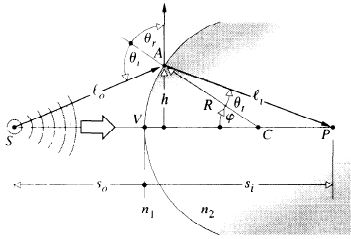
\includegraphics[scale=.75]{SphericalLens1.jpg}

S is the source, V is the vertex when the surface is closest to the point source along the optical axis (the optical axis follows line from S to V to C to P), h is the height of an incident ray from the optical axis when it hits the surface, R is the radius of the sphere, P is the point at which the ray becomes focused, A is the point at which the ray encounters the surface, $\theta_i, \theta_r, \theta_t$ are the angles of incidence, reflection, and transmission, $s_o$ is the object distance (simply the distance between the object and the lens) and $s_1$ is the image distance (distance from the edge of the lens to the focal point inside the lens). The optical path length in this case is: $OPL = n_1 l_0 + n_2 l_i$. 

Assuming that we are in the paraxial region ($\varphi$ is very small), we can simplify the distance relationships along the optical axis to: \[\frac{n_1}{s_o}+\frac{n_2}{s_i}=\frac{n_2-n_1}{R} \] which gives us the distance of the focal point or source when other geometries and material properties are known. 

\subsection{Thin Lenses}
There are various types of lenses. Thin lenses are considered to be so thin that their thickness is negligible.

\paragraph{Thin-Lens Equations}
The following image is used for the parameters in the thin lens equation: 

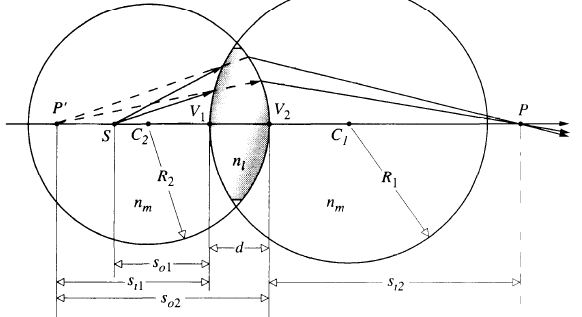
\includegraphics[scale=.75]{ThinLens.jpg}

This lens obviously has some thickness. For finding the s terms in the image, the geometrical analysis yields: \[\frac{n_m}{s_{o1}}+\frac{n_m}{s_{i2}} = (n_i-n_m)\left(\frac{1}{R_1}-\frac{1}{R_2}\right)+\frac{n_id}{(s_{i1}-d)s_{i1}} \]

As the distance d approaches zero (ie, the lens is thin) the equation takes the form of the Thin-Lens Equation (Lensmaker's Formula):
\begin{equation}
\frac{n_m}{s_{o1}}+\frac{n_m}{s_{i2}} = (n_i-n_m)\left(\frac{1}{R_1}-\frac{1}{R_2}\right)
\end{equation}

For a lens with an air interface, $n_m$ is approximately 1, so the equation often reads:
\[\frac{1}{s_{o1}}+\frac{1}{s_{i2}} = (n_i-1)\left(\frac{1}{R_1}-\frac{1}{R_2}\right)\]

If $s_o$ is moved out to infinity, the image distance becomes the focal length, $f_i$. Similarly, the object distance becomes the focal length $f_o$. In this case,, $f_i = f_o$ which leads to:
\begin{equation}
\frac{1}{f} = (n_l - 1)\left(\frac{1}{R_1}-\frac{1}{R_2}\right)
\end{equation}
and
\begin{equation}
\frac{1}{s_o}+\frac{1}{s_i} = \frac{1}{f}
\end{equation}
Which is the Gaussian Lens Formula. 

\paragraph{Focal Points and Planes}

The figure below shows where the focal point will lie for different types of lenses. The dark regions correspond the a higher index of refraction than the lighter regions. 

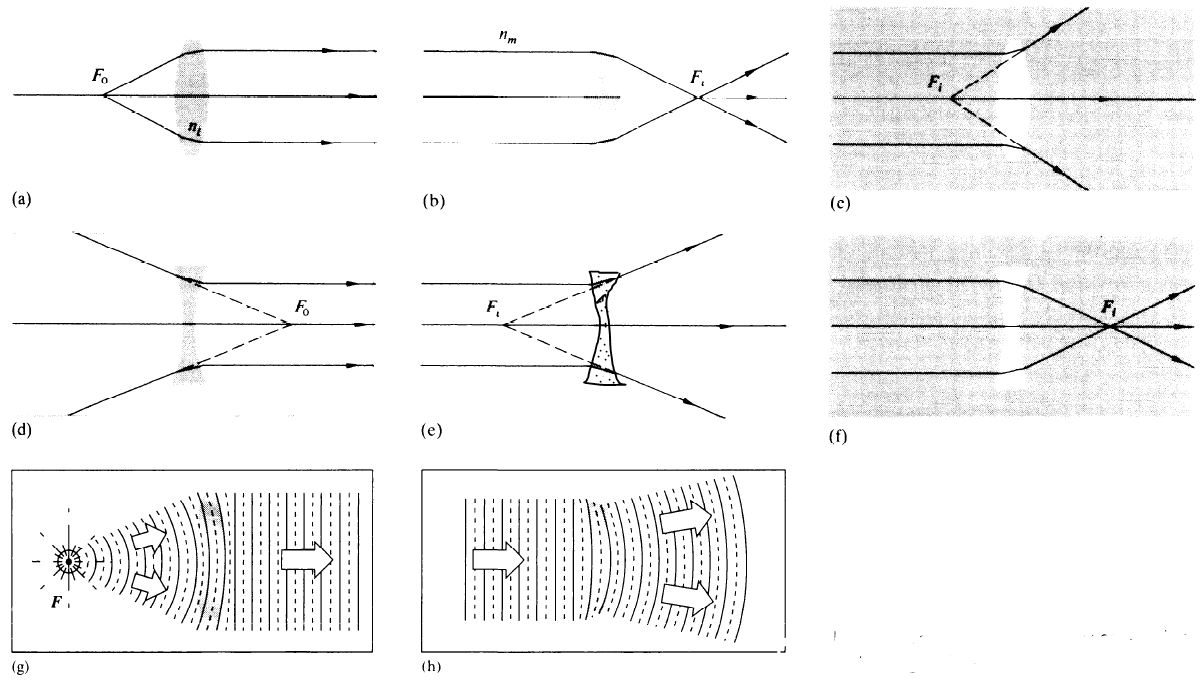
\includegraphics[scale=.45]{FocalPoint.jpg}

A focal plane is the plane in which a bundle of paraxial rays will all focus when passing through a lens. It can be visualized like so:

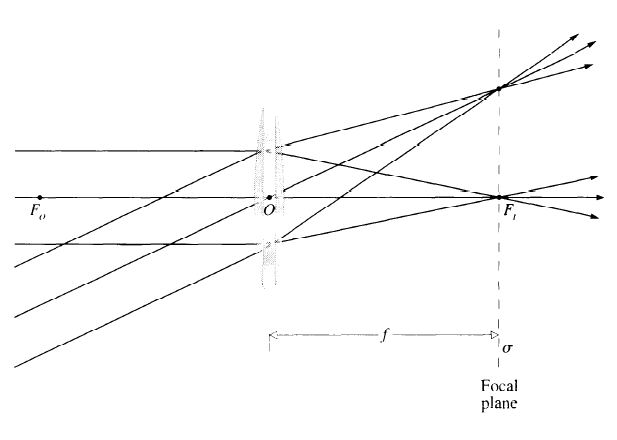
\includegraphics[scale=.75]{FocalPlane1.jpg}

\paragraph{Finite Imagery}

For imaging objects (not just points), we can approximate the object as having many point sources that approximately lie on a plane. The final image formed by a lens of a small planar object normal to the optical axis will itself be a small plane normal to that axis. See figure below:

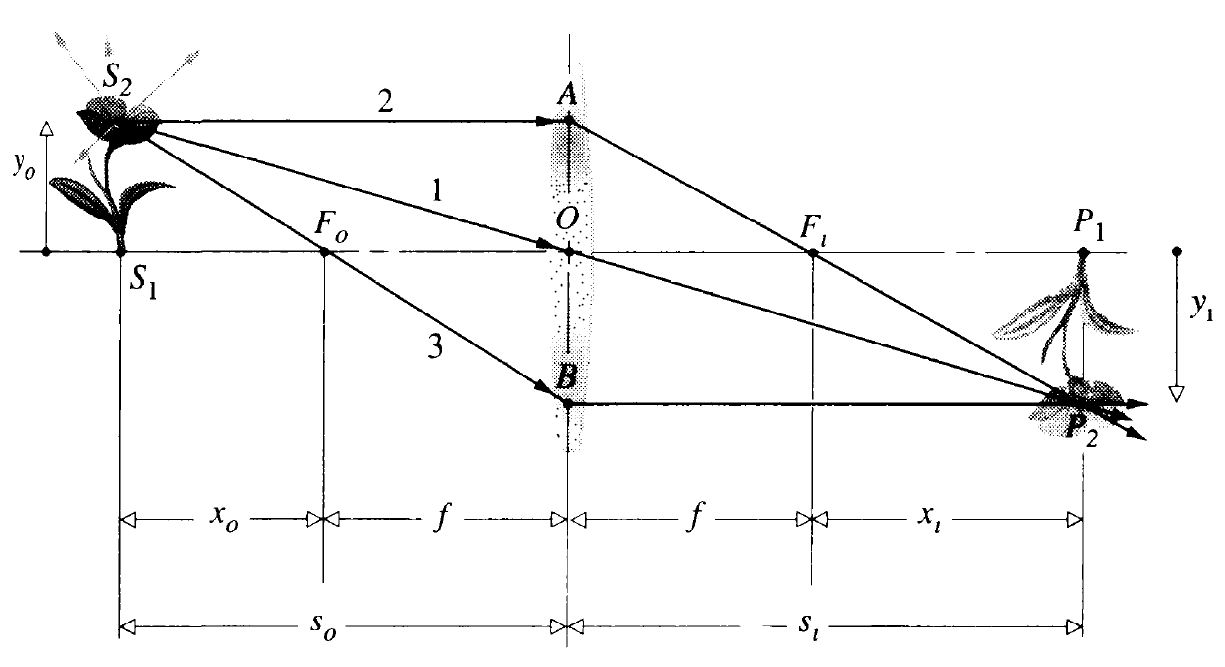
\includegraphics[scale=.4]{FiniteImagery.jpg}

The Newtonian form of the lens equation following this geometric scheme is: 
\begin{equation}
x_ox_i = f^2
\end{equation}
A fallout from this equation is that $x_o, x_i$ have like signs and thus: the object and image must be on opposite sides of their respective focal points. 

The lateral or transverse magnification, $M_T$ is the ratio of the transverse dimensions of the final image formed by an optical system to the corresponding dimension of the object. 
\begin{equation}
M_T \equiv \frac{y_i}{y_o} = -\frac{s_i}{s_o}
\end{equation}
A positive $M_T$ causes an erect image, a negatice inverts the image. All real images formed by a single thin lens will be inverted. 

Note that as an object approaches a lens, the real image moves away from it. 
\paragraph{Thin Lens Combinations}
A possible combination of thin lenses is shown below:

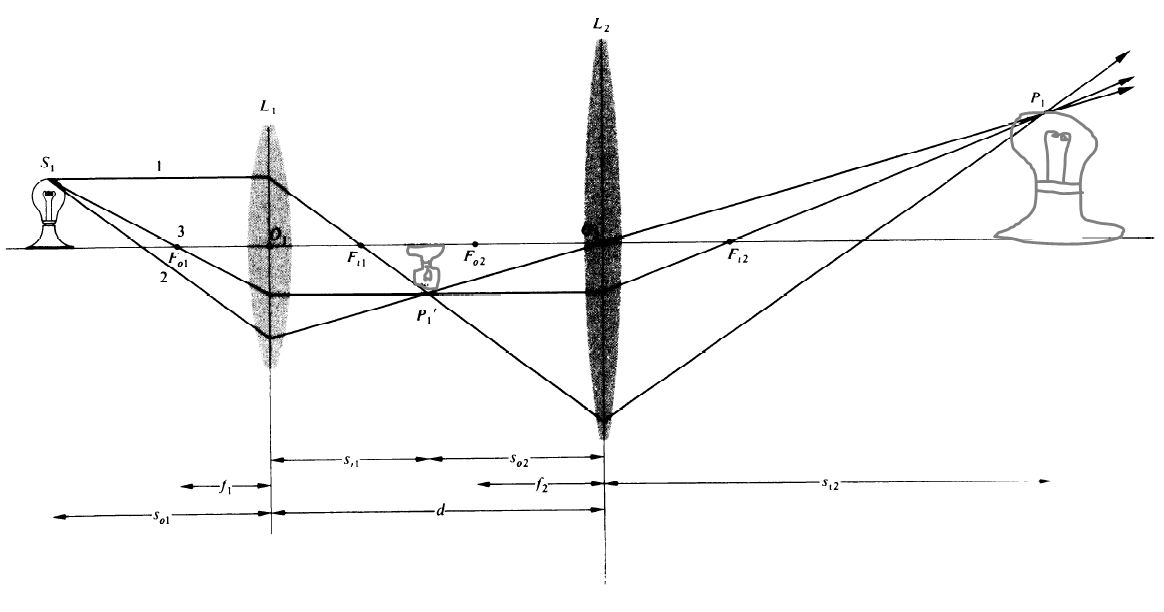
\includegraphics[scale=.45]{ThinLensCombo.jpg}

The distance from the last surface of an optical system to the second focal point of that system is the back focal length. The distance from the vertex of the first surface to the first object focus is the front focal length. For thin lenses, the back focal length equals the front focal length such that:
\[b.f.l = f. f.l = \frac{f_2f_1}{f_2+f_1}\]
The thin lens as an effective focal length, $f$ such that:
\begin{equation}
\frac{1}{f} = \frac{1}{f_1}+\frac{1}{f_2}
\end{equation}

\section{Stops}
\subsection{Aperture and Field Stops}
Any element that determines the amount of light reaching the image is known as an aperture stop (A.S.). An aperture stop can be the lens boundary itself or another sort of mechanism. These are used to limit the light in a system so that oblique rays are removed. The element limiting size or angular breadth of the object that can be imaged by the system is called the field stop (F.S). The field stop limits the field of view.  
\subsection{Entrance and Exit Pupils}
Entrance and exit pupils are images of an aperture stop. The entrance pupil of a system is the image of the aperture stop as seen from an axial point on the object through those elements preceding the stop. The exit pupil is the image of the aperture stop as seen from an axial point on the image plain through the interposed lenses if there are any. 

The chief ray is any ray from an off-axis object point that passes through the center of the aperture stop. The chief ray enters the optical system along a line directed toward the midpoint of the entrance pupil, $E_{np}$, and leaves the system along a line passing through the center of the exit pupil, $E_{xp}$ 

An illustration of an entrance pupil, an exit pupil, and a chief ray are below:

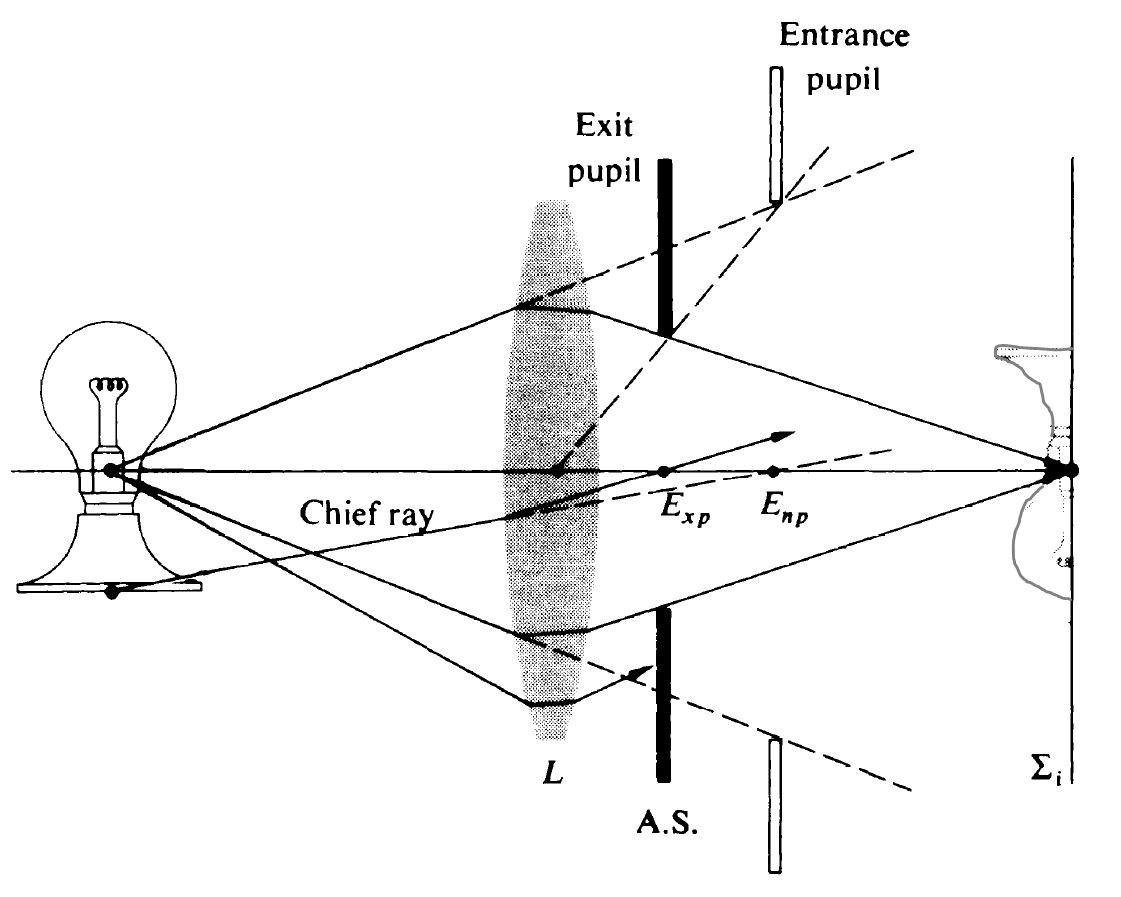
\includegraphics[scale=.25]{ChiefRay.jpg}

A marginal ray goes from the axial object point to the rim or margin of the entrance pupil (or aperture stop). When ray tracing, it is conventional to show both a chief ray and a marginal ray. Marginal rays are often dimmer than chief rays. This process of gradual fading out of the image at points near its periphery is a process called vignetting. 

\subsection{Relative Aperture and f-Number}
The flux density at an image plane varies as $(D/f)^2$. The ration $D/f$ is called the relative aperture. The inverse of the relative aperture is the focal ratio ($f$-number) commonly written as $f/\#$

\[f/\# = \equiv \frac{f}{D}\]

\section{Mirrors}
\subsection{Planar Mirrors}
Planar mirrors show an inverse image of the objects that they reflect. When a mirror is rotated by an angle $\alpha$ the angle of an incoming beam's incidence is altered by $2\alpha$.

\subsection{Aspherical Mirrors}
Aspherical mirrors can be used to shape light waves. Parabolic mirrors can be used to focus a plane wave onto a point. Mirrors also exist in hyperbolic and ellipsoid forms. Telescopes often use these geometries. 
\subsection{Spherical Mirrors}
Once again, spherical mirrors are cheaper than hyperbolic mirrors, but only function well under precise circumstances. The rest of the section goes into math involving the paraxial region of a spherical mirror and the formula that can be used within the paraxial region to calculate critical distances.

The Mirror Formula and the equations for the focal lengths are as follows:

\begin{equation}
\frac{1}{s_o}+\frac{1}{s_i} = -\frac{2}{R}
\end{equation}
\begin{equation}
f_o = f_i = -\frac{R}{2} 
\end{equation}
\begin{equation}
\frac{1}{s_o}+\frac{1}{s_i} = \frac{1}{f}
\end{equation}


An image of the geometry for this setup is:

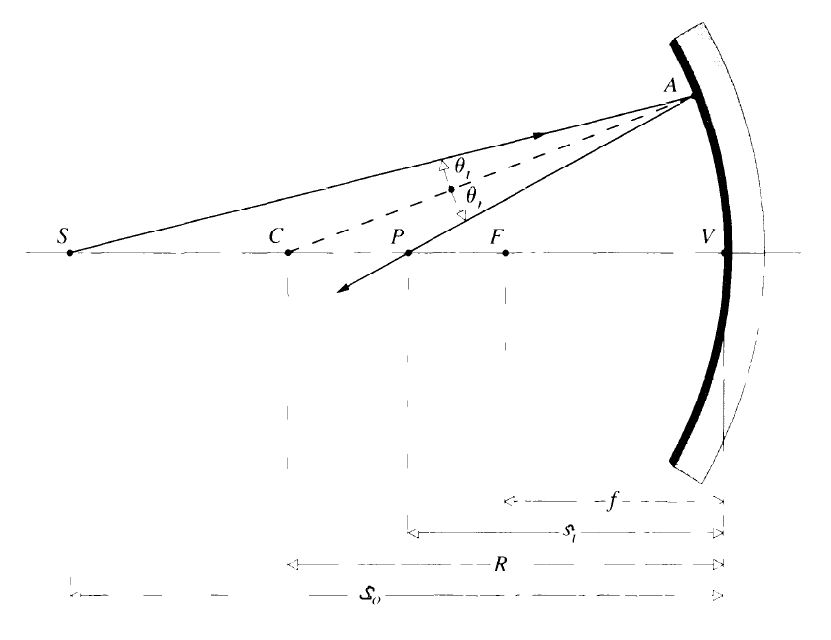
\includegraphics[scale=.5]{SphericalMirror.jpg}

$f$ is positive for concave mirrors and negative for convex mirrors. 

Mirrors form finite images similarly for lenses. The equations shown in that section are extremely similar. The only one with variation is that for transverse magnification which changes to: $y_i/y_o=-s_i/s_o$

\section{Prisms}
\subsection{Dispersing prisms}
A dispersing prism separates light into constituent frequencies through the process of dispersion. The angles involved in prism geometries can be illustrated in the following diagram:

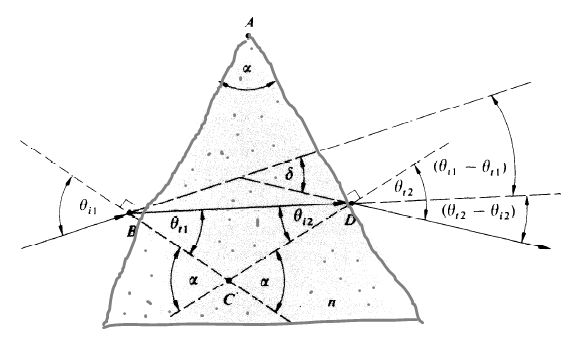
\includegraphics[scale=.5]{DispersingPrism.jpg}

Snell's law for the prism is:
\begin{equation}
n = \frac{\sin [(\delta_m+\alpha)/2]}{\sin \alpha/2}
\end{equation}
\subsection{Reflecting prisms}
Dispersion is not desirable in reflecting prisms. The main application of these guys is to move light around in a compact area. There are many types of reflecting prisms, all for different applications. Sometimes a face or faces must be silvered for the prism to work properly. 

\section{Optical Systems}

\subsection{The compound microscope}
The compound microscope is a device that uses short focal length objective lenses to magnify objects nearby. A real, inverted image is produced and then magnified further by eyepieces that act as magnifying glasses. 


\subsection{The telescope}
Refracting light telescopes strongly resemble compount microscopes. The main difference is that they focus on objects that are very far away. Increasing the aperture diameter can increase the resolution of a telescope. Large lenses are difficult to manufacture, however so light-gathering mirrors (which are much easier to manufacture) are used instead in the form of reflecting telescopes. 


\section{Glossary}
\begin{description}
\item[Aberration: ] An image error. Happens when using spherical lenses.
\item[Achromatic: ] A prisim is said to be achromatic if the reflection inside it will occur without any color preferences. 
\item[Angular deviation (wrt prisms): ]
\item[Aperture / field stop: ] An object that limits the light rays that can travel through the system (aperture stop) or limits the field of view of the image (field stop). 
\item[Aspheric: ] Optical elements that have one or both surfaces as neither planar nor spherical. 
\item[Chief ray: ] The chief ray is any ray fron an off-axis object point that passes through the center of the aperture stop. The chief ray enters the optical system along a line directed toward the midpoint of the entrance pupil, $E_{np}$, and leaves the system along a line passing through the center of the exit pupil, $E_{xp}$
\item[Collimated: ] Parallel rays.
\item[Concave: ] describes lenses that are thinner in the middle than on the edges. 
\item[Conjugate point: ] A point in an optical system which can be used to image or can be imaged by another point. The Principle of Reversibility allows for such a point to be equally well imaged from another point and vice versa. 
\item[Converging lens: ] A lens that causes the incoming beam to converge, bending it more toward the central axis (usually convex lenses).
\item[Convex: ] When lenses are thicker at their midpoints than at their edges. 
\item[Diffraction-limited: ] An optical system limited by the fundamental limit on the degree of perfection of an optical system as is set by diffraction. 
\item[Dispersing prism: ] A dispersing prism separates light into constituent frequencies through the process of dispersion. (dispersion is the material property that makes objects have indices of refraction that are variable with wavelength)
\item[Diverging lens: ] A lens that turns rays outward away from the central axis (usually concave lenses)
\item[Entrance/exit pupil: ] The entrance pupil of a system is the image of the aperture stop as seen from an axial point on the object through those elements preceding the stop. The exit pupil is the image of the aperture stop as seen from an axial point on the image plain through the interposed lenses if there are any. 
\item[Erect image: ] an image that is not inverted. It has the same orientation as the object that is being imaged. 
\item[F-number: ] The ratio of focal length to aperture. 
\item[Focal plane: ] The plane in which a bundle of paraxial rays will all focus when passing through a lens. 
\item[Front/back focal length: ] The distance from the last surface of an optical system to the second focal point of that system is the back focal length. The distance from the vertex of the first surface to the first object focus is the front focal length. 
\item[Geometrical Optics: ] The process in which the subject treats the controlled manipulation of wave-fronts (or rays) by means of the interpositioning of reflecting and/or refracting bodies, neglecting any diffraction effects. 
\item[Inverted image: ] When an image's y value (measured upward from the optical axis) changes sign when traveling through an optical system. 
\item[Lens: ] A lens is a refracting device (ie: a discontinuity in the prevailing medium) that reconfigures a transmitted energy distribution.
\item[Lensmaker's formula: ] The equation describing a thin lens in air: $\frac{1}{s_{o1}}+\frac{1}{s_{i2}} = (n_i-1)\left(\frac{1}{R_1}-\frac{1}{R_2}\right) $
\item[Longitudinal magnification: ] Not the same as transverse magnification. The longitudinal magnification is the magnification in the axial direction. 
\item[Marginal ray: ] A marginal ray goes from the axial object point to the rim or margin of the entrance pupil (or aperture stop). 
\item[Optical axis: ] The central axis of an optical system / spherical lens.
\item[Paraxial ray: ] Rays that arrive at shallow angles on a lens with respect to the optical axis. These will form a perfect image of an object S at point P on the optical axis. 
\item[Real image: ] An image formed by converging rays. 
\item[Reflecting prism: ] A reflecting prism functions to change the orientation of an image or in the direction of propagation in a beam. They are not dispersive. 
\item[Vignetting: ] The gradual fading out of the image at points near its periphery. 
\item[Virtual image: ] An image that would be made at the equivalent focal point for diverging rays. 

\end{description}

\section{Useful Equations}
\[\frac{n_m}{s_{o1}}+\frac{n_m}{s_{i2}} = (n_i-n_m)\left(\frac{1}{R_1}-\frac{1}{R_2}\right)\]
\[\frac{1}{f} = (n_l - 1)\left(\frac{1}{R_1}-\frac{1}{R_2}\right)\]
\[\frac{1}{s_o}+\frac{1}{s_i} = \frac{1}{f}\]
\[x_ox_i = f^2\]
\[M_T \equiv \frac{y_i}{y_o} = -\frac{s_i}{s_o}\]
\[\frac{1}{f} = \frac{1}{f_1}+\frac{1}{f_2}\]
\[\frac{1}{s_o}+\frac{1}{s_i} = -\frac{2}{R}\]
\[f_o = f_i = -\frac{R}{2} \]
\[n = \frac{\sin [(\delta_m+\alpha)/2]}{\sin \alpha/2}\]


\chapter{More on Geometrical Optics}
\chapter{Fourier Optics}


\end{document}
